% Options for packages loaded elsewhere
\PassOptionsToPackage{unicode}{hyperref}
\PassOptionsToPackage{hyphens}{url}
\PassOptionsToPackage{dvipsnames,svgnames,x11names}{xcolor}
%
\documentclass[
  letterpaper,
  DIV=11,
  numbers=noendperiod]{scrartcl}

\usepackage{amsmath,amssymb}
\usepackage{iftex}
\ifPDFTeX
  \usepackage[T1]{fontenc}
  \usepackage[utf8]{inputenc}
  \usepackage{textcomp} % provide euro and other symbols
\else % if luatex or xetex
  \usepackage{unicode-math}
  \defaultfontfeatures{Scale=MatchLowercase}
  \defaultfontfeatures[\rmfamily]{Ligatures=TeX,Scale=1}
\fi
\usepackage{lmodern}
\ifPDFTeX\else  
    % xetex/luatex font selection
\fi
% Use upquote if available, for straight quotes in verbatim environments
\IfFileExists{upquote.sty}{\usepackage{upquote}}{}
\IfFileExists{microtype.sty}{% use microtype if available
  \usepackage[]{microtype}
  \UseMicrotypeSet[protrusion]{basicmath} % disable protrusion for tt fonts
}{}
\makeatletter
\@ifundefined{KOMAClassName}{% if non-KOMA class
  \IfFileExists{parskip.sty}{%
    \usepackage{parskip}
  }{% else
    \setlength{\parindent}{0pt}
    \setlength{\parskip}{6pt plus 2pt minus 1pt}}
}{% if KOMA class
  \KOMAoptions{parskip=half}}
\makeatother
\usepackage{xcolor}
\setlength{\emergencystretch}{3em} % prevent overfull lines
\setcounter{secnumdepth}{5}
% Make \paragraph and \subparagraph free-standing
\ifx\paragraph\undefined\else
  \let\oldparagraph\paragraph
  \renewcommand{\paragraph}[1]{\oldparagraph{#1}\mbox{}}
\fi
\ifx\subparagraph\undefined\else
  \let\oldsubparagraph\subparagraph
  \renewcommand{\subparagraph}[1]{\oldsubparagraph{#1}\mbox{}}
\fi

\usepackage{color}
\usepackage{fancyvrb}
\newcommand{\VerbBar}{|}
\newcommand{\VERB}{\Verb[commandchars=\\\{\}]}
\DefineVerbatimEnvironment{Highlighting}{Verbatim}{commandchars=\\\{\}}
% Add ',fontsize=\small' for more characters per line
\usepackage{framed}
\definecolor{shadecolor}{RGB}{241,243,245}
\newenvironment{Shaded}{\begin{snugshade}}{\end{snugshade}}
\newcommand{\AlertTok}[1]{\textcolor[rgb]{0.68,0.00,0.00}{#1}}
\newcommand{\AnnotationTok}[1]{\textcolor[rgb]{0.37,0.37,0.37}{#1}}
\newcommand{\AttributeTok}[1]{\textcolor[rgb]{0.40,0.45,0.13}{#1}}
\newcommand{\BaseNTok}[1]{\textcolor[rgb]{0.68,0.00,0.00}{#1}}
\newcommand{\BuiltInTok}[1]{\textcolor[rgb]{0.00,0.23,0.31}{#1}}
\newcommand{\CharTok}[1]{\textcolor[rgb]{0.13,0.47,0.30}{#1}}
\newcommand{\CommentTok}[1]{\textcolor[rgb]{0.37,0.37,0.37}{#1}}
\newcommand{\CommentVarTok}[1]{\textcolor[rgb]{0.37,0.37,0.37}{\textit{#1}}}
\newcommand{\ConstantTok}[1]{\textcolor[rgb]{0.56,0.35,0.01}{#1}}
\newcommand{\ControlFlowTok}[1]{\textcolor[rgb]{0.00,0.23,0.31}{#1}}
\newcommand{\DataTypeTok}[1]{\textcolor[rgb]{0.68,0.00,0.00}{#1}}
\newcommand{\DecValTok}[1]{\textcolor[rgb]{0.68,0.00,0.00}{#1}}
\newcommand{\DocumentationTok}[1]{\textcolor[rgb]{0.37,0.37,0.37}{\textit{#1}}}
\newcommand{\ErrorTok}[1]{\textcolor[rgb]{0.68,0.00,0.00}{#1}}
\newcommand{\ExtensionTok}[1]{\textcolor[rgb]{0.00,0.23,0.31}{#1}}
\newcommand{\FloatTok}[1]{\textcolor[rgb]{0.68,0.00,0.00}{#1}}
\newcommand{\FunctionTok}[1]{\textcolor[rgb]{0.28,0.35,0.67}{#1}}
\newcommand{\ImportTok}[1]{\textcolor[rgb]{0.00,0.46,0.62}{#1}}
\newcommand{\InformationTok}[1]{\textcolor[rgb]{0.37,0.37,0.37}{#1}}
\newcommand{\KeywordTok}[1]{\textcolor[rgb]{0.00,0.23,0.31}{#1}}
\newcommand{\NormalTok}[1]{\textcolor[rgb]{0.00,0.23,0.31}{#1}}
\newcommand{\OperatorTok}[1]{\textcolor[rgb]{0.37,0.37,0.37}{#1}}
\newcommand{\OtherTok}[1]{\textcolor[rgb]{0.00,0.23,0.31}{#1}}
\newcommand{\PreprocessorTok}[1]{\textcolor[rgb]{0.68,0.00,0.00}{#1}}
\newcommand{\RegionMarkerTok}[1]{\textcolor[rgb]{0.00,0.23,0.31}{#1}}
\newcommand{\SpecialCharTok}[1]{\textcolor[rgb]{0.37,0.37,0.37}{#1}}
\newcommand{\SpecialStringTok}[1]{\textcolor[rgb]{0.13,0.47,0.30}{#1}}
\newcommand{\StringTok}[1]{\textcolor[rgb]{0.13,0.47,0.30}{#1}}
\newcommand{\VariableTok}[1]{\textcolor[rgb]{0.07,0.07,0.07}{#1}}
\newcommand{\VerbatimStringTok}[1]{\textcolor[rgb]{0.13,0.47,0.30}{#1}}
\newcommand{\WarningTok}[1]{\textcolor[rgb]{0.37,0.37,0.37}{\textit{#1}}}

\providecommand{\tightlist}{%
  \setlength{\itemsep}{0pt}\setlength{\parskip}{0pt}}\usepackage{longtable,booktabs,array}
\usepackage{calc} % for calculating minipage widths
% Correct order of tables after \paragraph or \subparagraph
\usepackage{etoolbox}
\makeatletter
\patchcmd\longtable{\par}{\if@noskipsec\mbox{}\fi\par}{}{}
\makeatother
% Allow footnotes in longtable head/foot
\IfFileExists{footnotehyper.sty}{\usepackage{footnotehyper}}{\usepackage{footnote}}
\makesavenoteenv{longtable}
\usepackage{graphicx}
\makeatletter
\def\maxwidth{\ifdim\Gin@nat@width>\linewidth\linewidth\else\Gin@nat@width\fi}
\def\maxheight{\ifdim\Gin@nat@height>\textheight\textheight\else\Gin@nat@height\fi}
\makeatother
% Scale images if necessary, so that they will not overflow the page
% margins by default, and it is still possible to overwrite the defaults
% using explicit options in \includegraphics[width, height, ...]{}
\setkeys{Gin}{width=\maxwidth,height=\maxheight,keepaspectratio}
% Set default figure placement to htbp
\makeatletter
\def\fps@figure{htbp}
\makeatother

% load packages
\usepackage{geometry}
\usepackage{xcolor}
\usepackage{eso-pic}
\usepackage{fancyhdr}
\usepackage{sectsty}
\usepackage{fontspec}
\usepackage{titlesec}

%% Set page size with a wider right margin
\geometry{a4paper, total={170mm,257mm}, left=20mm, top=20mm, bottom=20mm, right=50mm}

%% Let's define some colours
\definecolor{uniblue}{HTML}{003865}
\definecolor{burgundy}{HTML}{7D2239}
\definecolor{cobalt}{HTML}{005C8A}
\definecolor{lavender}{HTML}{5B4D94}
\definecolor{leaf}{HTML}{006630}
\definecolor{moss}{HTML}{385A4F}
\definecolor{pillarbox}{HTML}{B30C00}
\definecolor{rust}{HTML}{9A3A06}
\definecolor{sandstone}{HTML}{52473B}
\definecolor{skyblue}{HTML}{005398}
\definecolor{slate}{HTML}{4F5961}
\definecolor{thistle}{HTML}{951272}

%\definecolor{light}{HTML}{E6E6FA} % original from template - redefined below as uni blue at 10 percent:
\colorlet{light}{uniblue!10}
%\definecolor{highlight}{HTML}{800080} % original from template - redefined below as uni's skyblue:
\colorlet{highlight}{skyblue}
%\definecolor{dark}{HTML}{330033} % original from template - redefined below as uni blue at 100 percent:
\colorlet{dark}{uniblue}

%% Let's add the border on the right hand side 
\AddToShipoutPicture{% 
    \AtPageLowerLeft{% 
        \put(\LenToUnit{\dimexpr\paperwidth-3cm},0){% 
            \color{light}\rule{3cm}{\LenToUnit\paperheight}%
          }%
     }%
     % logo
    \AtPageLowerLeft{% start the bar at the bottom right of the page
        \put(\LenToUnit{\dimexpr\paperwidth-2.25cm},27.2cm){% move it to the top right
            \color{light}
\includegraphics[width=2.25cm]{_extensions/nrennie/PrettyPDF/uni_logo_boxed.jpg}
          }%
     }%
}

%% Style the page number
\fancypagestyle{mystyle}{
  \fancyhf{}
  \renewcommand\headrulewidth{0pt}
  \fancyfoot[R]{\thepage}
  \fancyfootoffset{3.5cm}
}
\setlength{\footskip}{20pt}

%% style the chapter/section fonts
\chapterfont{\color{uniblue}\fontsize{20}{16.8}\selectfont}
\sectionfont{\color{uniblue}\fontsize{20}{16.8}\selectfont}
\subsectionfont{\color{skyblue}\fontsize{14}{16.8}\selectfont}
\titleformat{\subsection}
  {\color{uniblue!90}\sffamily\Large\bfseries}{\thesubsection}{1em}{}[{\titlerule[0.8pt]}]
\subsubsectionfont{\color{cobalt}}

\renewcommand\thesection{\color{slate}\arabic{section}}
  
% left align title
\makeatletter
\renewcommand{\maketitle}{\bgroup\setlength{\parindent}{0pt}
\begin{flushleft}
  {\color{uniblue}\sffamily\huge\textbf{\@title}} \vspace{0.3cm} \newline
  {\Large {\@subtitle}} \newline
  \@author
\end{flushleft}\egroup
}
\makeatother

%% Use some custom fonts
\setsansfont{Ubuntu}[
    Path=_extensions/nrennie/PrettyPDF/Ubuntu/,
    Scale=0.9,
    Extension = .ttf,
    UprightFont=*-Regular,
    BoldFont=*-Bold,
    ItalicFont=*-Italic,
    ]

\setmainfont{Ubuntu}[
    Path=_extensions/nrennie/PrettyPDF/Ubuntu/,
    Scale=0.9,
    Extension = .ttf,
    UprightFont=*-Regular,
    BoldFont=*-Bold,
    ItalicFont=*-Italic,
    ]
\KOMAoption{captions}{tableheading}
\makeatletter
\@ifpackageloaded{tcolorbox}{}{\usepackage[skins,breakable]{tcolorbox}}
\@ifpackageloaded{fontawesome5}{}{\usepackage{fontawesome5}}
\definecolor{quarto-callout-color}{HTML}{909090}
\definecolor{quarto-callout-note-color}{HTML}{0758E5}
\definecolor{quarto-callout-important-color}{HTML}{CC1914}
\definecolor{quarto-callout-warning-color}{HTML}{EB9113}
\definecolor{quarto-callout-tip-color}{HTML}{00A047}
\definecolor{quarto-callout-caution-color}{HTML}{FC5300}
\definecolor{quarto-callout-color-frame}{HTML}{acacac}
\definecolor{quarto-callout-note-color-frame}{HTML}{4582ec}
\definecolor{quarto-callout-important-color-frame}{HTML}{d9534f}
\definecolor{quarto-callout-warning-color-frame}{HTML}{f0ad4e}
\definecolor{quarto-callout-tip-color-frame}{HTML}{02b875}
\definecolor{quarto-callout-caution-color-frame}{HTML}{fd7e14}
\makeatother
\makeatletter
\@ifpackageloaded{caption}{}{\usepackage{caption}}
\AtBeginDocument{%
\ifdefined\contentsname
  \renewcommand*\contentsname{Table of contents}
\else
  \newcommand\contentsname{Table of contents}
\fi
\ifdefined\listfigurename
  \renewcommand*\listfigurename{List of Figures}
\else
  \newcommand\listfigurename{List of Figures}
\fi
\ifdefined\listtablename
  \renewcommand*\listtablename{List of Tables}
\else
  \newcommand\listtablename{List of Tables}
\fi
\ifdefined\figurename
  \renewcommand*\figurename{Figure}
\else
  \newcommand\figurename{Figure}
\fi
\ifdefined\tablename
  \renewcommand*\tablename{Table}
\else
  \newcommand\tablename{Table}
\fi
}
\@ifpackageloaded{float}{}{\usepackage{float}}
\floatstyle{ruled}
\@ifundefined{c@chapter}{\newfloat{codelisting}{h}{lop}}{\newfloat{codelisting}{h}{lop}[chapter]}
\floatname{codelisting}{Listing}
\newcommand*\listoflistings{\listof{codelisting}{List of Listings}}
\makeatother
\makeatletter
\makeatother
\makeatletter
\@ifpackageloaded{caption}{}{\usepackage{caption}}
\@ifpackageloaded{subcaption}{}{\usepackage{subcaption}}
\makeatother
\makeatletter
\@ifpackageloaded{tcolorbox}{}{\usepackage[skins,breakable]{tcolorbox}}
\makeatother
\makeatletter
\@ifundefined{shadecolor}{\definecolor{shadecolor}{rgb}{.97, .97, .97}}{}
\makeatother
\makeatletter
\@ifundefined{codebgcolor}{\definecolor{codebgcolor}{named}{light}}{}
\makeatother
\makeatletter
\ifdefined\Shaded\renewenvironment{Shaded}{\begin{tcolorbox}[colback={codebgcolor}, frame hidden, enhanced, breakable, boxrule=0pt, sharp corners]}{\end{tcolorbox}}\fi
\makeatother
\ifLuaTeX
  \usepackage{selnolig}  % disable illegal ligatures
\fi
\usepackage{bookmark}

\IfFileExists{xurl.sty}{\usepackage{xurl}}{} % add URL line breaks if available
\urlstyle{same} % disable monospaced font for URLs
\hypersetup{
  pdftitle={Collaborative Coding 2},
  colorlinks=true,
  linkcolor={highlight},
  filecolor={Maroon},
  citecolor={Blue},
  urlcolor={highlight},
  pdfcreator={LaTeX via pandoc}}

\title{Collaborative Coding 2}
\author{}
\date{}

\begin{document}
\maketitle

\pagestyle{mystyle}

This week's material is based on the \textbf{Version Control Course}
from the School of Mathematics and Statistics from the University of
Glasgow. The content has been reduced to fit the class structure.
However, we do encourage you to take a look and attempt the full course.
Please get in touch if you would like to get access the full course.

\section{Add collaborator}\label{add-collaborator}

To collaborate with users in a repository that belongs to your personal
account on GitHub.com, you can
\href{https://docs.github.com/en/account-and-profile/setting-up-and-managing-your-personal-account-on-github/managing-access-to-your-personal-repositories/inviting-collaborators-to-a-personal-repository}{invite
the users as collaborators}.

\section{Clone}\label{clone}

One way to download a project to your computer is to use Git's
\texttt{clone} method. To use \texttt{clone}, we need to tell Git
installed on our computer to make a copy (or `clone') of another
repository, in this case from GitHub.

Clone is a Git feature that allows a user to make a copy of a
repository, including all the associated metadata on their computer so
they can work on it. This is an essential feature and makes sense for a
team of collaborators, with read-and-write privileges to the repository,
all working on a project together.

\subsection{Command-line}

First, we need to copy the address of the repository we want to clone.

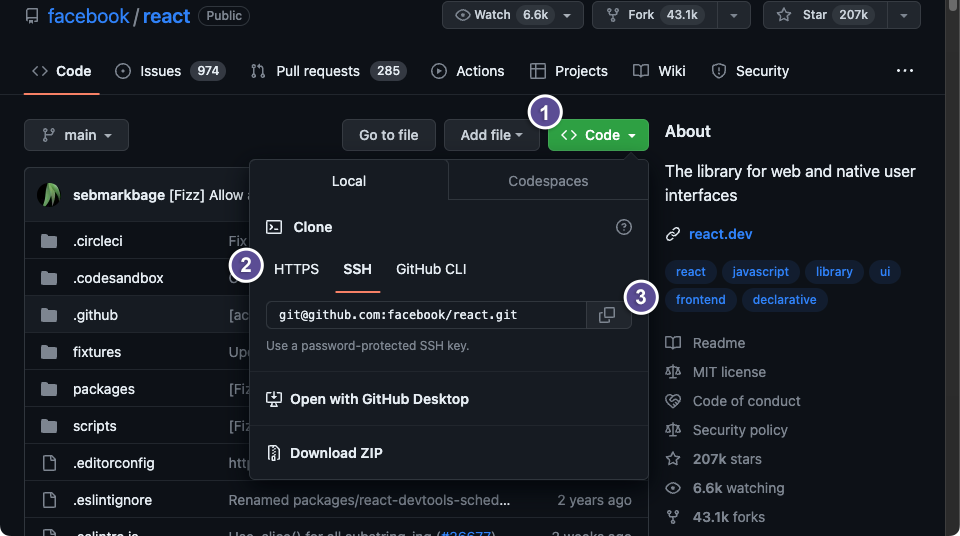
\includegraphics{images/image23.png}

\begin{enumerate}
\def\labelenumi{\arabic{enumi}.}
\item
  Click on the green button labelled ``Code''
\item
  Choose either HTTPS or SSH, depending on how you connect to GitHub
  with Git on your computer (see the Configuration section of Unit 1)
\item
  Copy the address
\end{enumerate}

Then in your terminal, navigate to your desired folder and issue the
following command:

\begin{Shaded}
\begin{Highlighting}[]
\NormalTok{git clone }\SpecialCharTok{\textless{}}\NormalTok{address}\SpecialCharTok{\textgreater{}}
\end{Highlighting}
\end{Shaded}

You should now see the repository has been cloned to your computer.

\subsection{GitHub Desktop}

First, navigate to the repository you want to clone on the GitHub
website.

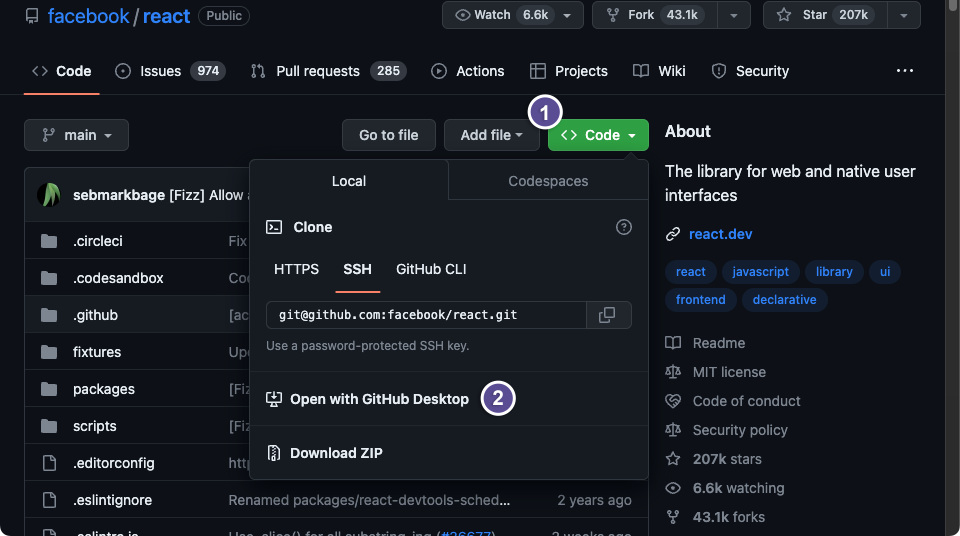
\includegraphics{images/image24.png}

\begin{enumerate}
\def\labelenumi{\arabic{enumi}.}
\item
  Click on the green button labelled `Code'
\item
  Click on `Open with GitHub Desktop'
\item
  You should then see a window like this pop up in GitHub Desktop:
\end{enumerate}

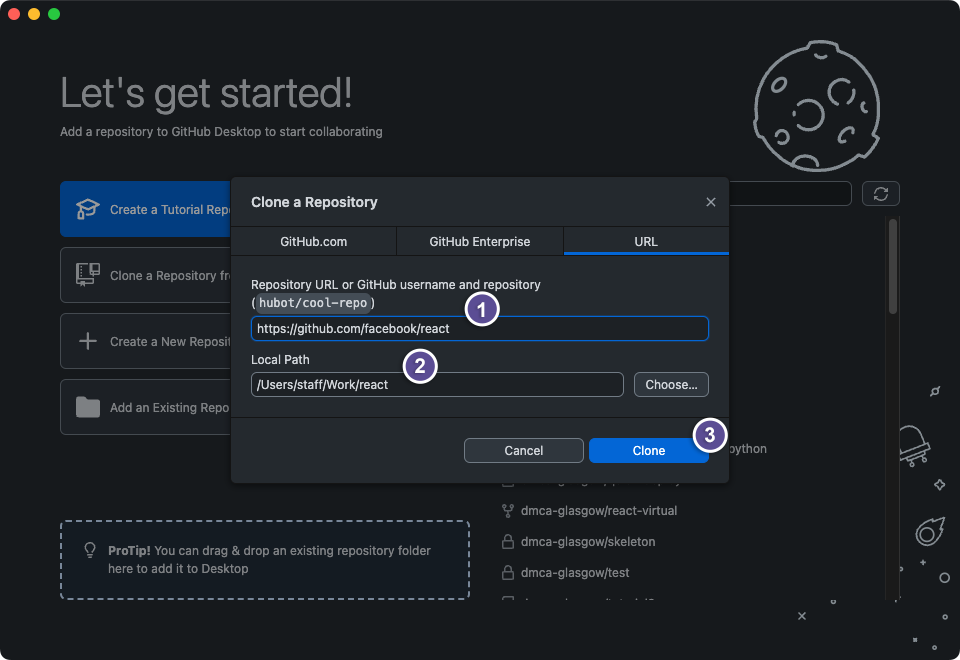
\includegraphics{images/image25.png}

\begin{enumerate}
\def\labelenumi{\arabic{enumi}.}
\item
  The URL of the repository on GitHub has automatically been populated
\item
  Choose where you would like the repository to be cloned to on your
  computer
\item
  Click `Clone'
\end{enumerate}

Using this approach, we have a copy of the files and folders in the
repository, but we have also copied the metadata which makes this into a
Git repository. To answer the example above, now if a project maintainer
makes an update to the project on GitHub, we can easily sync both
versions:

\subsection{Command-line}

In the project folder just issue the \texttt{pull} command:

\begin{Shaded}
\begin{Highlighting}[]
\NormalTok{git pull}
\end{Highlighting}
\end{Shaded}

\subsection{GitHub Desktop}

On GitHub Desktop, click the `Fetch origin' button in the top bar:

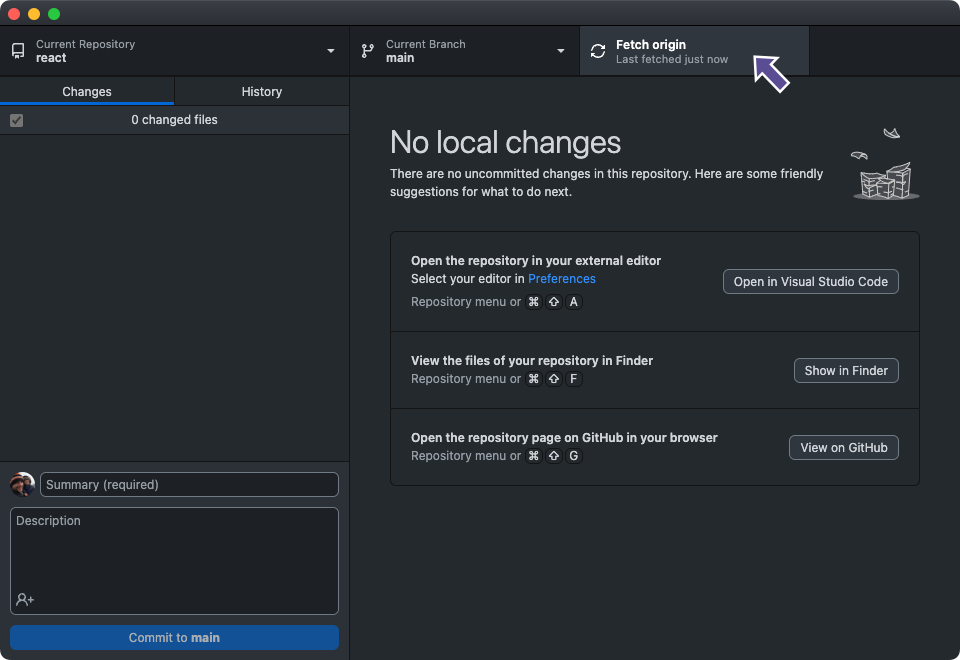
\includegraphics{images/image26.png}

\section{Branching and branching
strategies}\label{branching-and-branching-strategies}

\subsection{Introduction}\label{introduction}

Typically a project will have one main direction of development--- to
reach a predetermined goal, such as a fully working prototype or to
complete a course assessment. When Git uses the analogy of a tree (with
branches), this main direction could be thought of as the `trunk' of
your development flow.

So far, we have only committed changes to one branch, the default branch
called \texttt{main}, which, in our tree analogy, can be thought of as
the trunk. If you are working on your own, or with a small group and you
are not all committing changes at the same time, this can be a valid
approach and avoids a lot of complexity in using Git.

Branches allow you to `branch off' from the trunk in a new direction,
which we may then add back to our trunk at a later time (see next
paragraph). On this new branch, you can experiment with new ideas or
work away in isolation, committing to Git and pushing your changes to
GitHub, safe in the knowledge that nothing you do will affect the main
direction of development. Likewise, the main direction of development on
\texttt{main} can carry on in parallel with its own changes, and these
will not affect your isolated branch.

It's possible to \textbf{merge} the changes made in a branch, into
another branch (usually the \texttt{main} branch). For example, if you
created a branch to try out an experiment and the experiment was a
success, Git enables you to merge those changes back into the main
branch, or main direction of development, then you can delete your
branch as it's no longer needed. Or, if the experiment failed, you can
leave the branch and never speak of it again, although it will still be
stored if you decide later it is a good idea after all, or you can
safely delete the branch.

Similarly, you can merge the changes from`\texttt{main} into your
branch. This is useful if, for example, \texttt{main} has had updates
made to it since you `branched off', and you would like to see these
updates in your branch.

Git offers another method to merge branches called \textbf{rebase},
which is why the Git term for merging branches is \textbf{integration}
as this covers both methods. Although rebase has some advantages, you
can risk losing work when using it, so it won't be covered in this
course.

\subsection{Motivation}\label{motivation}

\subsubsection{Working with other
people}\label{working-with-other-people}

Branches enable a team to work on the same files at the same time.
However, it doesn't work like other collaboration tools like Google Docs
or Microsoft 365, where you can see other users editing parts of a file
as you work. Instead, branches allow collaborators to work in isolation,
not worrying about what others are up to, and when the time comes to
\textbf{integrate} changes into the default branch, Git provides the
tools to ensure you don't overwrite someone else's work (or, if you do,
you do it very intentionally!).

\subsubsection{Grouping commits}\label{grouping-commits}

Even if you're working on your own, branches can be used as a tool to
group multiple commits. For example, when working on a new feature for a
project, you can create a branch named after your feature, then continue
to use Git best practices by \textbf{breaking your task into small
manageable chunks}, and \textbf{complete one thing at a time and commit
it}. Then when it comes time to integrate your changes to the main
branch, you can choose to ``squash'' those small commits down into one
``merge commit'' named after your new feature. This helps to keep the
commit history on the default branch minimal and tidy, only showing
completed tasks such as new features and bug fixes.

\section{Branching and integrating}\label{branching-and-integrating}

This week we are going to learn how to create a branch and make changes
to it, then integrate this branch back into the \texttt{main} branch.
This is particularly helpful when working collaboratively.

In Git, a branch represents a distinct version of the \texttt{main}
repository, serving as a snapshot of your changes. When implementing new
features or addressing issues, regardless of their scope, creating a new
branch is the practice to isolate your modifications. This approach
enhances code stability in the main branch and affords you the
opportunity to refine your history before merging it into the primary
codebase.

When the work is complete, a branch can be merged with the main project.
You can even switch between branches and work on different projects
without them interfering with each other.

We are also going to learn about Git's stash feature, and how it can
help you when switching between branches.

\subsection{Create a new local Git
repository}\label{create-a-new-local-git-repository}

Let's create a new folder on our computer called `tutorial3' and
initialise Git:

\subsection{Command-line}

Create a directory for your `tutorial3' work:

\begin{Shaded}
\begin{Highlighting}[]
\NormalTok{mkdir tutorial3}
\NormalTok{cd tutorial3}
\end{Highlighting}
\end{Shaded}

and run git init inside:

\begin{Shaded}
\begin{Highlighting}[]
\NormalTok{git init}
\end{Highlighting}
\end{Shaded}

\begin{verbatim}

Initialized empty Git repository in /Users/staff/Work/tutorial3/.git/
\end{verbatim}

\subsection{GitHub Desktop}

Choose \texttt{File\ \textgreater{}\ New\ Repository...} from the menu.

In the ``Create a New Repository'' form, name the repository
``tutorial3'', set the ``Local Path'' field to your preferred location
and click the ``Create Repository'' button:

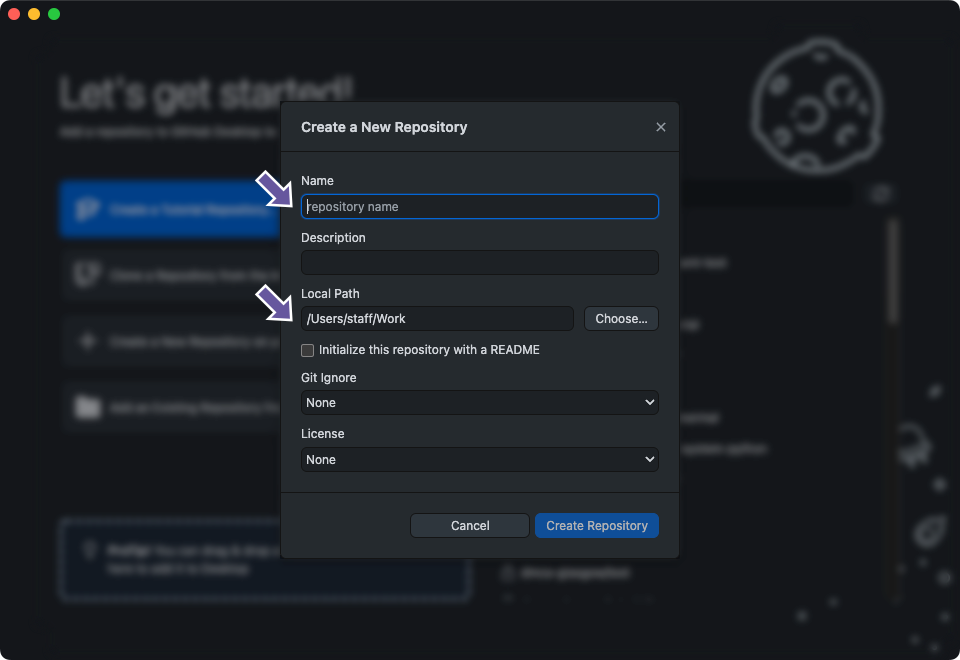
\includegraphics{images/image27.png}

Add the following file to the repository:

\begin{tcolorbox}[enhanced jigsaw, opacityback=0, colframe=quarto-callout-note-color-frame, toprule=.15mm, arc=.35mm, rightrule=.15mm, title=\textcolor{quarto-callout-note-color}{\faInfo}\hspace{0.5em}{example.md}, colbacktitle=quarto-callout-note-color!10!white, left=2mm, leftrule=.75mm, opacitybacktitle=0.6, toptitle=1mm, colback=white, bottomtitle=1mm, breakable, titlerule=0mm, bottomrule=.15mm, coltitle=black]

Hello

\end{tcolorbox}

Then add and commit the file:

\subsection{Command-line}

\begin{Shaded}
\begin{Highlighting}[]
\NormalTok{git add example.md}
\NormalTok{git commit }\SpecialCharTok{{-}}\NormalTok{m }\StringTok{"Add example.md"}
\end{Highlighting}
\end{Shaded}

\subsection{GitHub Desktop}

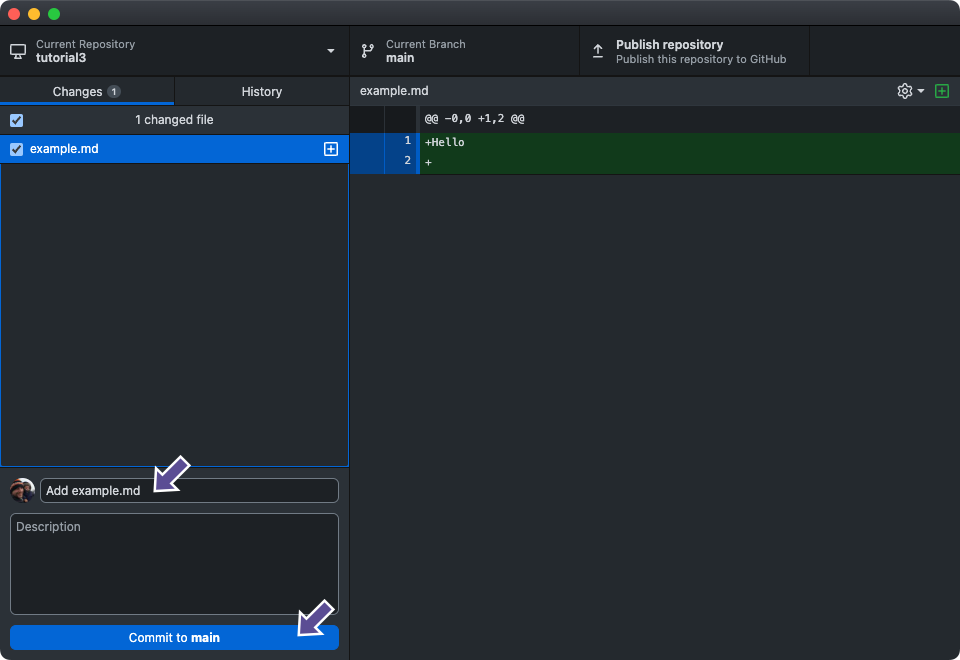
\includegraphics{images/image28.png}

Next, let's create a branch named \texttt{shout} based on this commit.

\subsection{Command-line}

We can create a new branch and switch to it using the switch command
with the -c flag:

\begin{Shaded}
\begin{Highlighting}[]
\NormalTok{git }\ControlFlowTok{switch} \SpecialCharTok{{-}}\NormalTok{c shout}
\end{Highlighting}
\end{Shaded}

\begin{verbatim}

Switched to a new branch 'shout'
\end{verbatim}

\subsection{GitHub Desktop}

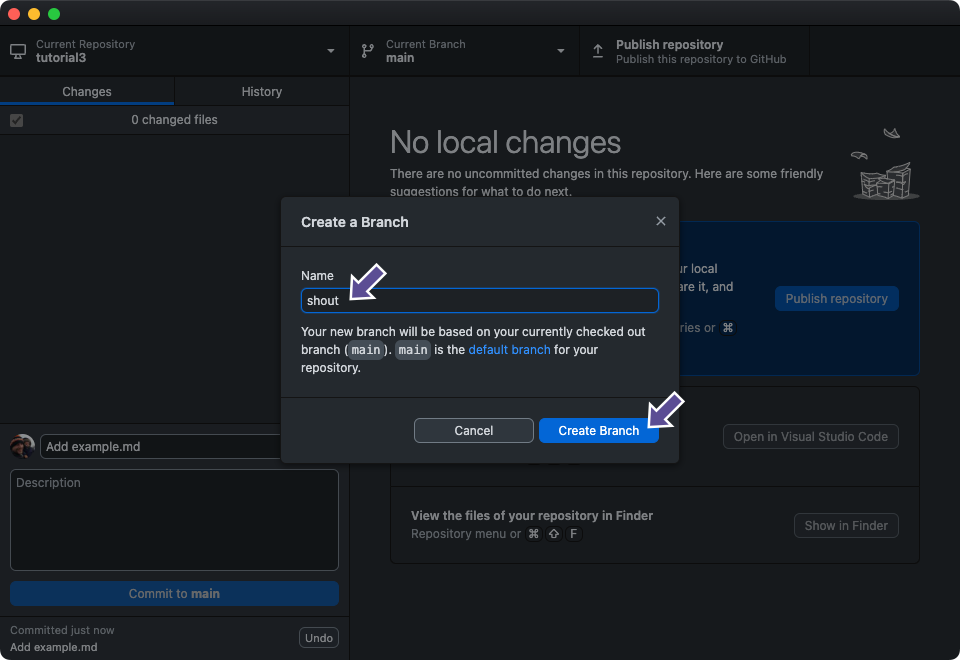
\includegraphics{images/image29.png}

Add an exclamation mark to the end of the word within the
\texttt{example.md} file:

\begin{tcolorbox}[enhanced jigsaw, opacityback=0, colframe=quarto-callout-note-color-frame, toprule=.15mm, arc=.35mm, rightrule=.15mm, title=\textcolor{quarto-callout-note-color}{\faInfo}\hspace{0.5em}{example.md}, colbacktitle=quarto-callout-note-color!10!white, left=2mm, leftrule=.75mm, opacitybacktitle=0.6, toptitle=1mm, colback=white, bottomtitle=1mm, breakable, titlerule=0mm, bottomrule=.15mm, coltitle=black]

Hello!

\end{tcolorbox}

Then commit the change:

\subsection{Command-line}

\begin{Shaded}
\begin{Highlighting}[]
\NormalTok{git add example.md}
\end{Highlighting}
\end{Shaded}

\begin{verbatim}

git commit -m "Add exclamation mark"

[shout eed4222] Add exclamation mark

1 file changed, 1 insertion(+), 1 deletion(-)
\end{verbatim}

\subsection{GitHub Desktop}

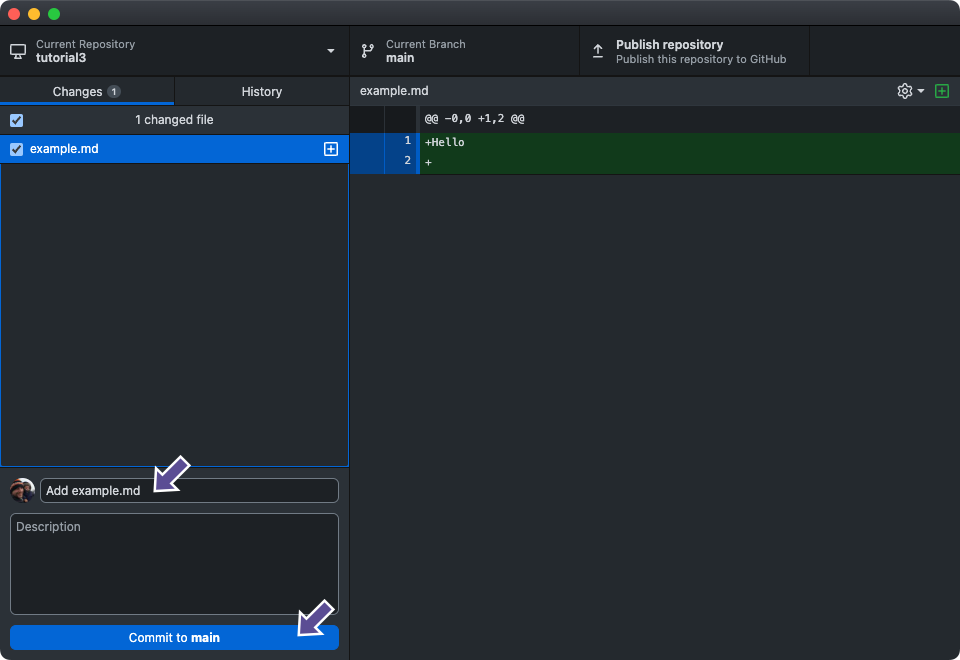
\includegraphics{images/image30.png}

Let's take a quick look at the log:

\subsection{Command-line}

\begin{Shaded}
\begin{Highlighting}[]
\NormalTok{git log }\SpecialCharTok{{-}{-}}\NormalTok{all }\SpecialCharTok{{-}{-}}\NormalTok{decorate }\SpecialCharTok{{-}{-}}\NormalTok{oneline }\SpecialCharTok{{-}{-}}\NormalTok{graph}
\end{Highlighting}
\end{Shaded}

\begin{verbatim}

* eed4222 (HEAD -> shout) Add exclamation mark

* 8f601cd (main) Add example.md
\end{verbatim}

\subsection{GitHub Desktop}

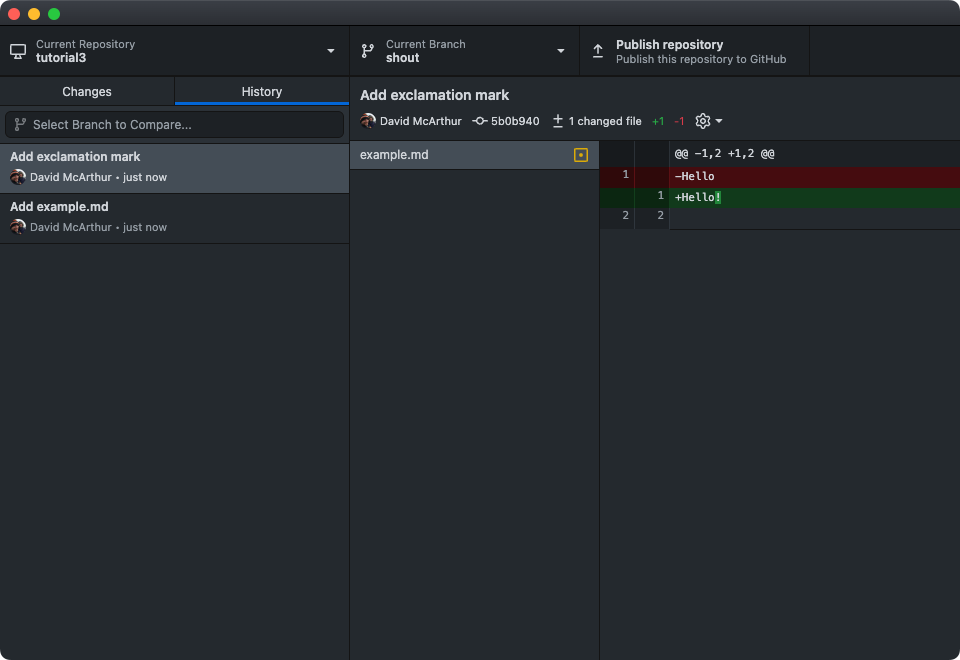
\includegraphics{images/image31.png}

Now let's try merging the branch back into the \texttt{main} branch.
First, switch back to \texttt{main}:

\subsection{Command-line}

\begin{Shaded}
\begin{Highlighting}[]
\NormalTok{git }\ControlFlowTok{switch}\NormalTok{ main}
\end{Highlighting}
\end{Shaded}

\begin{verbatim}

Switched to branch 'main'
\end{verbatim}

(Note, we don't include the -c flag as this branch already exists)

\subsection{GitHub Desktop}

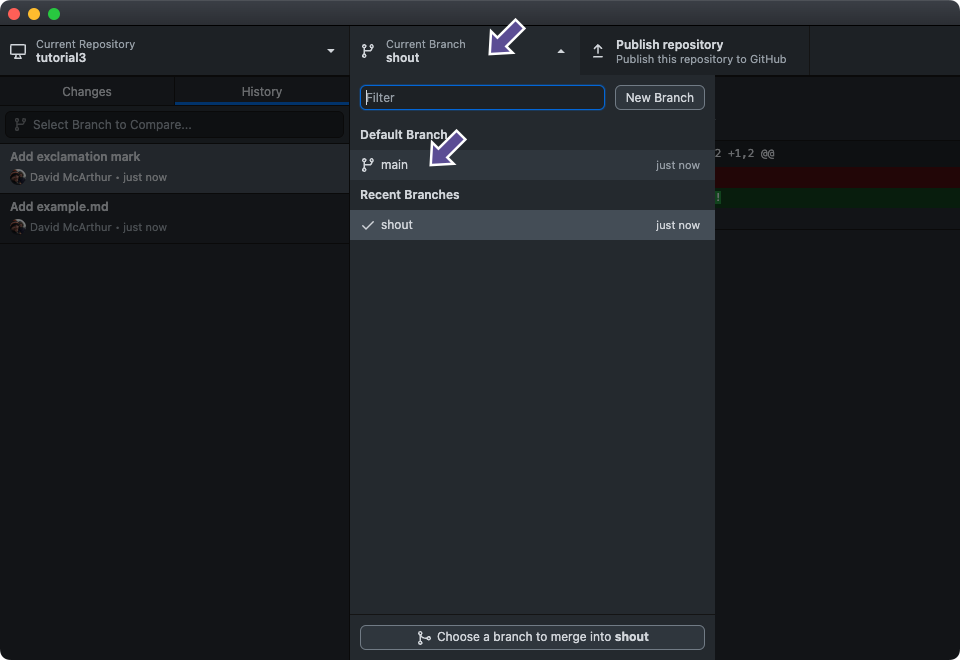
\includegraphics{images/image32.png}

Then merge our \texttt{shout} branch into \texttt{main}:

\subsection{Command-line}

\begin{Shaded}
\begin{Highlighting}[]
\NormalTok{git merge shout}
\end{Highlighting}
\end{Shaded}

\begin{verbatim}

Updating 8f601cd..eed4222

Fast-forward

example.md | 2 +-

1 file changed, 1 insertion(+), 1 deletion(-)
\end{verbatim}

\subsection{GitHub Desktop}

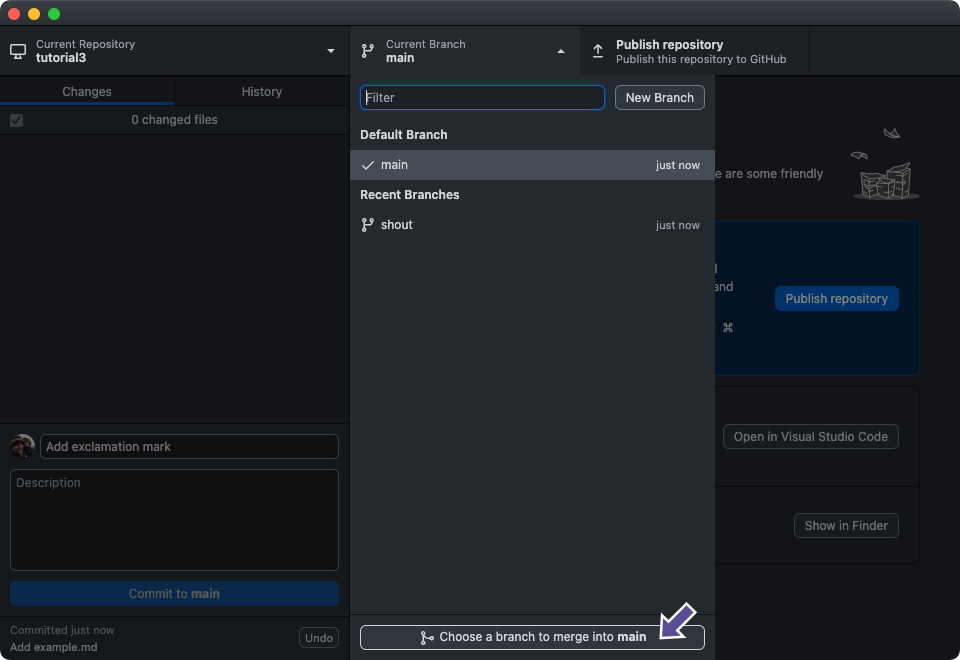
\includegraphics{images/image33.png}

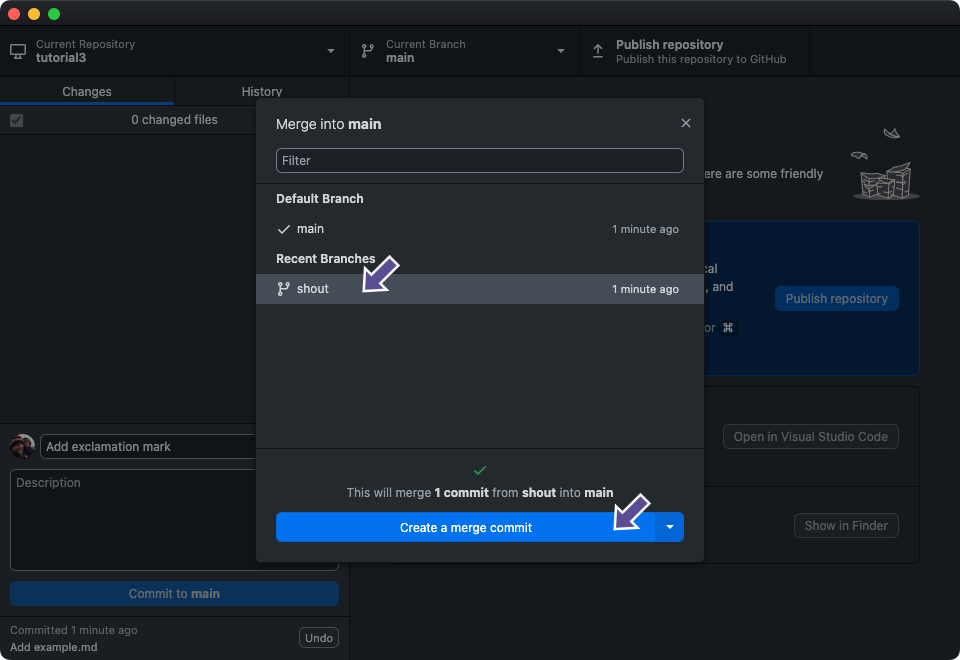
\includegraphics{images/image34.png}

We can check that the version of our file in the main branch now has the
exclamation mark:

\subsection{Command-line}

\begin{Shaded}
\begin{Highlighting}[]
\NormalTok{cat example.md}
\end{Highlighting}
\end{Shaded}

\begin{verbatim}

Hello!
\end{verbatim}

\subsection{GitHub Desktop}

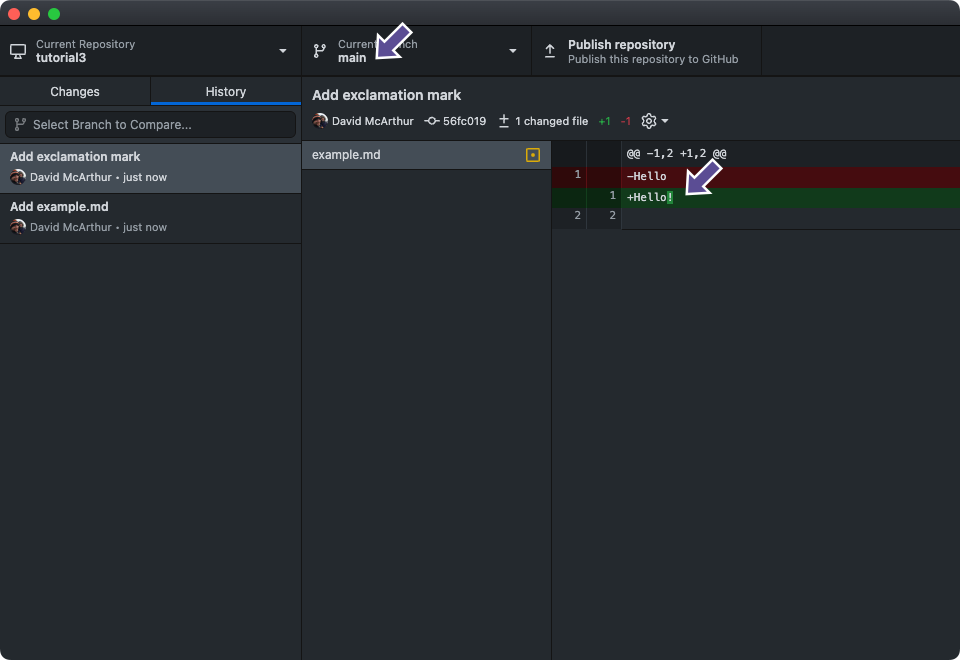
\includegraphics{images/image35.png}

As the change is now reflected in our \texttt{main} branch, we can
safely delete our \texttt{shout} branch:

\subsection{Command-line}

\begin{Shaded}
\begin{Highlighting}[]
\NormalTok{git branch }\SpecialCharTok{{-}{-}}\NormalTok{delete shout}
\end{Highlighting}
\end{Shaded}

\begin{verbatim}

Deleted branch shout (was eed4222).
\end{verbatim}

\subsection{GitHub Desktop}

Simply right click on the \texttt{shout} branch here and select Delete

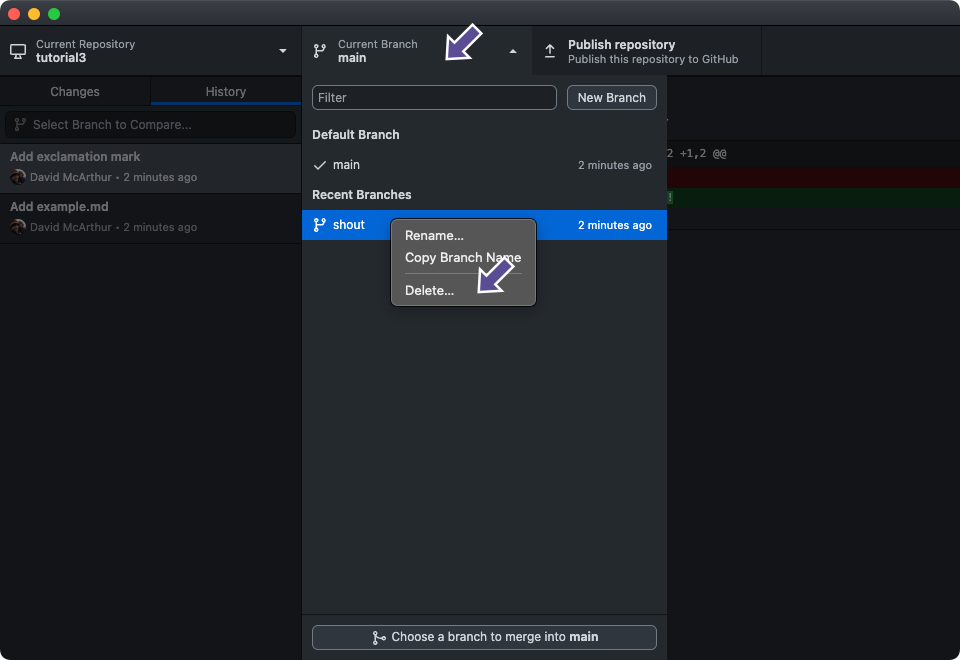
\includegraphics{images/image36.png}

\subsection{Switching branches with the help of Git
stash}\label{switching-branches-with-the-help-of-git-stash}

Given the example above, branching with Git appears straightforward.
However, this is not always the case. Sometimes Git won't let you switch
branches. Let's create a scenario where we see an error when switching
branches, try to understand why Git is stopping us, and look at a simple
universal solution.

Create and switch to a new branch called \texttt{question}:

\subsection{Command-line}

\begin{Shaded}
\begin{Highlighting}[]
\NormalTok{git }\ControlFlowTok{switch} \SpecialCharTok{{-}}\NormalTok{c question}
\end{Highlighting}
\end{Shaded}

\begin{verbatim}

Switched to a new branch 'question'
\end{verbatim}

\subsection{GitHub Desktop}

From the main menu select Branch \textgreater{} New Branch and name the
branch `question':

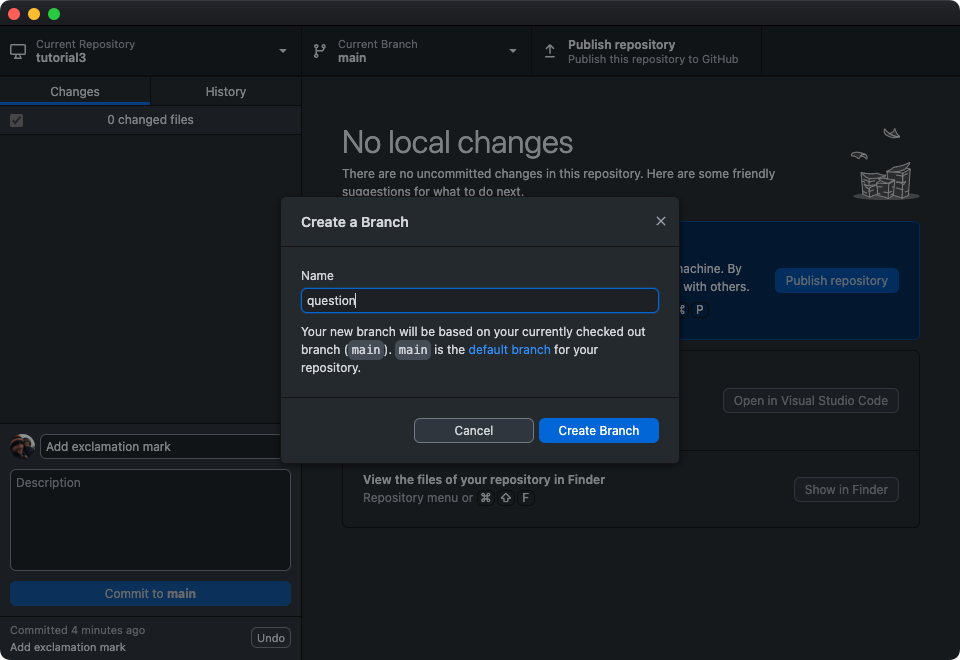
\includegraphics{images/image37.png}

Let's make a change to the file by changing the exclamation mark to a
question mark:

\begin{tcolorbox}[enhanced jigsaw, opacityback=0, colframe=quarto-callout-note-color-frame, toprule=.15mm, arc=.35mm, rightrule=.15mm, title=\textcolor{quarto-callout-note-color}{\faInfo}\hspace{0.5em}{example.md}, colbacktitle=quarto-callout-note-color!10!white, left=2mm, leftrule=.75mm, opacitybacktitle=0.6, toptitle=1mm, colback=white, bottomtitle=1mm, breakable, titlerule=0mm, bottomrule=.15mm, coltitle=black]

Hello?

\end{tcolorbox}

Add the change to the stage and commit:

\subsection{Command-line}

\begin{Shaded}
\begin{Highlighting}[]
\NormalTok{git add example.md}
\NormalTok{git commit }\SpecialCharTok{{-}}\NormalTok{m }\StringTok{"Change exclamation mark to question mark"}
\end{Highlighting}
\end{Shaded}

\begin{verbatim}
[question 49806f4] Change exclamation mark to question mark

1 file changed, 1 insertion(+), 1 deletion(-)
\end{verbatim}

\subsection{GitHub Desktop}

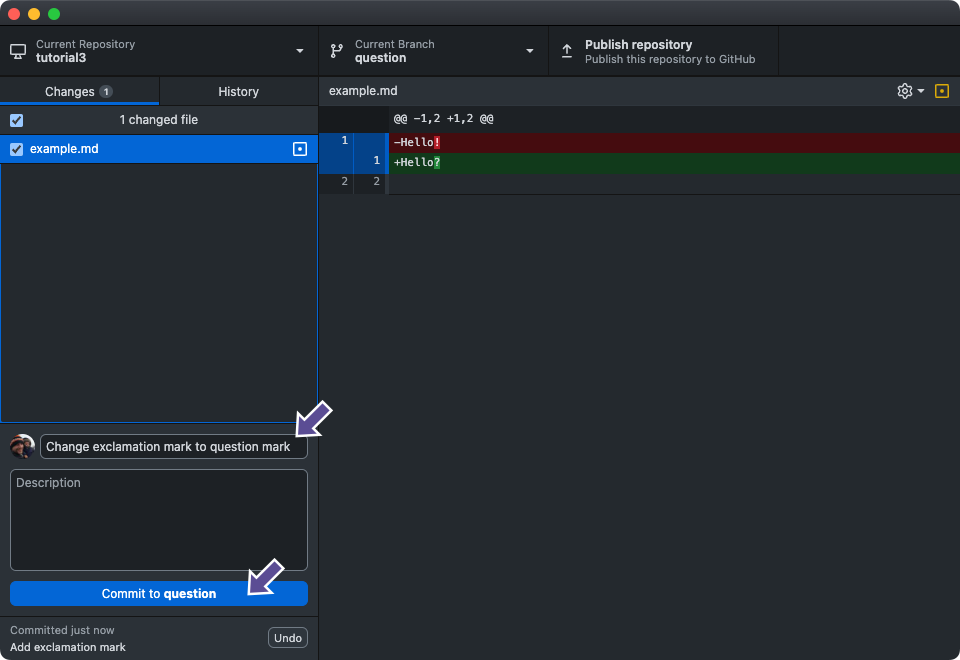
\includegraphics{images/image38.png}

Now let's make another change to our file:

\begin{tcolorbox}[enhanced jigsaw, opacityback=0, colframe=quarto-callout-note-color-frame, toprule=.15mm, arc=.35mm, rightrule=.15mm, title=\textcolor{quarto-callout-note-color}{\faInfo}\hspace{0.5em}{example.md}, colbacktitle=quarto-callout-note-color!10!white, left=2mm, leftrule=.75mm, opacitybacktitle=0.6, toptitle=1mm, colback=white, bottomtitle=1mm, breakable, titlerule=0mm, bottomrule=.15mm, coltitle=black]

Hello?

Is it me you're looking for?

\end{tcolorbox}

This time, instead of committing, we will try to switch back to the main
branch, and Git will tell us we can't switch branches currently as we
would lose our local changes (see the next example for the error).
Committing our latest change would let us then switch the branch, but
what if we don't want to commit the change?

\subsection{Command-line}

A common scenario is that you have started working on a problem, then
when you check Git you realise you are working on the wrong branch, but
now you have uncommitted changes and can't switch branches. For this
scenario, there is the \textbf{stash}. Think of it as a clipboard with
cut-and-paste functionality like you would have in a text editor, which
will let us `cut' our changes and store them somewhere safe, let us
switch branches, and then paste them.

Let's try it now:

\begin{Shaded}
\begin{Highlighting}[]
\NormalTok{git }\ControlFlowTok{switch}\NormalTok{ main}
\end{Highlighting}
\end{Shaded}

\begin{verbatim}

error: Your local changes to the following files would be overwritten by checkout:

example.md

Please commit your changes or stash them before you switch branches.

Aborting
\end{verbatim}

Git complains that we will lose our local changes. Let's try out the
stash:

\begin{Shaded}
\begin{Highlighting}[]
\NormalTok{git stash}
\end{Highlighting}
\end{Shaded}

\begin{verbatim}

Saved working directory and index state WIP on question: 49806f4 Change exclamation mark to question mark
\end{verbatim}

Git has used the abbreviation `WIP' which stands for `Work In Progress'.

Now if we look at our file we'll see the 2nd line has disappeared:

\begin{Shaded}
\begin{Highlighting}[]
\NormalTok{cat example.md}
\end{Highlighting}
\end{Shaded}

\begin{verbatim}

Hello?
\end{verbatim}

We can ask Git to show us our stash:

\begin{Shaded}
\begin{Highlighting}[]
\NormalTok{git stash show}
\end{Highlighting}
\end{Shaded}

\begin{verbatim}

example.md | 2 ++

1 file changed, 2 insertions(+)
\end{verbatim}

This shows us which files have changed. We can add a \texttt{-p} (for
`patch') flag which will show us a diff:

\begin{Shaded}
\begin{Highlighting}[]
\NormalTok{git stash show }\SpecialCharTok{{-}}\NormalTok{p}
\end{Highlighting}
\end{Shaded}

\begin{verbatim}

diff --git a/example.md b/example.md

index ebbc6cd..472b4c5 100644

--- a/example.md

+++ b/example.md

@@ -1,2 +1,4 @@

Hello?

+Is it me you're looking for?

+
\end{verbatim}

Now our local copy is `clean' and we can safely switch branches:

\begin{Shaded}
\begin{Highlighting}[]
\NormalTok{git }\ControlFlowTok{switch}\NormalTok{ main}
\end{Highlighting}
\end{Shaded}

\begin{verbatim}
Switched to branch 'main'
\end{verbatim}

And we can apply our change to a different branch:

\begin{Shaded}
\begin{Highlighting}[]
\NormalTok{git stash apply}
\end{Highlighting}
\end{Shaded}

\begin{verbatim}

Auto-merging example.md

On branch main

Changes not staged for commit:

(use "git add <file>..." to update what will be committed)

(use "git restore <file>..." to discard changes in working directory)

modified:   example.md

no changes added to commit (use "git add" and/or "git commit -a")
\end{verbatim}

And now if we look at the file, we'll see our stashed change has been
applied, but there is no question mark on ``Hello?'' as this change
still resides on the \texttt{question} branch:

\begin{Shaded}
\begin{Highlighting}[]
\NormalTok{cat example.md}
\end{Highlighting}
\end{Shaded}

\begin{verbatim}

Hello!

Is it me you're looking for?
\end{verbatim}

We can now safely remove our stashed version:

\begin{Shaded}
\begin{Highlighting}[]
\NormalTok{git stash drop}
\end{Highlighting}
\end{Shaded}

\begin{verbatim}

Dropped refs/stash@{0} (00b8825ce0b6a0e3c2877f3c42c828fb4da4c922)
\end{verbatim}

It's important to \texttt{drop} the stash afterwards, or you'll end up
with several items in the stash that could lead to applying the wrong
one. Git has a shortcut for `apply then drop' which is
\texttt{git\ stash\ pop}.

\subsection{GitHub Desktop}

Luckily for GitHub Desktop users, this stashing and stash-applying
process is all handled by clicking a button.

Once we try to switch to the \texttt{main} branch:

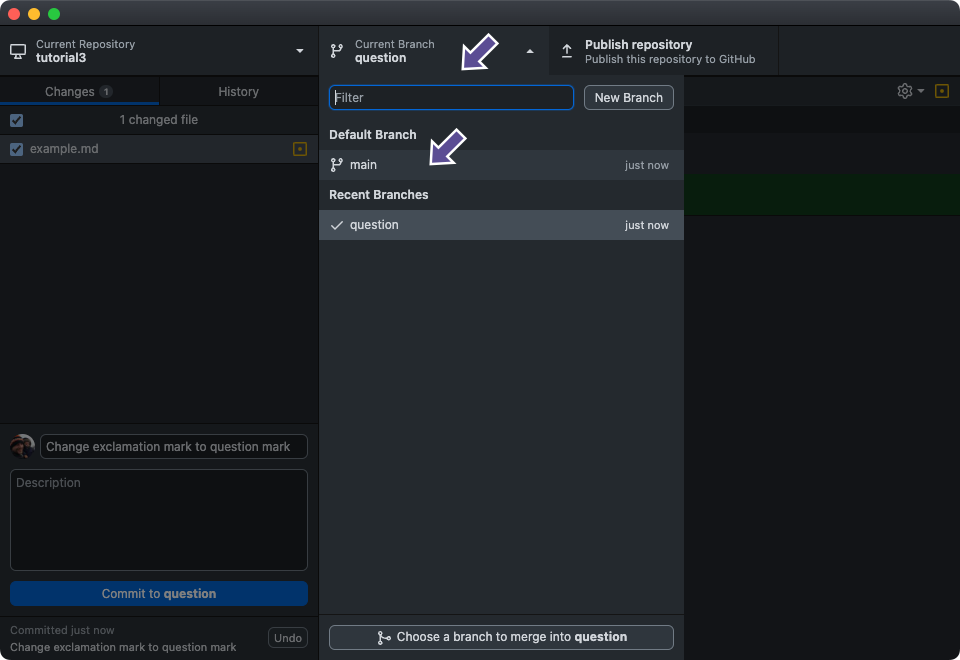
\includegraphics{images/image39.png}

GitHub Desktop offers us two options:

\begin{itemize}
\item
  \textbf{Leave my changes on question} allows us to stash the changes
  and come back to the branch later and apply the stash
\item
  \textbf{Bring my changes to main} automates the process of stashing
  the changes, switching to the desired branch, and applying the stash.
\end{itemize}

For this tutorial, we will choose the latter option--- `Bring my changes
to main':

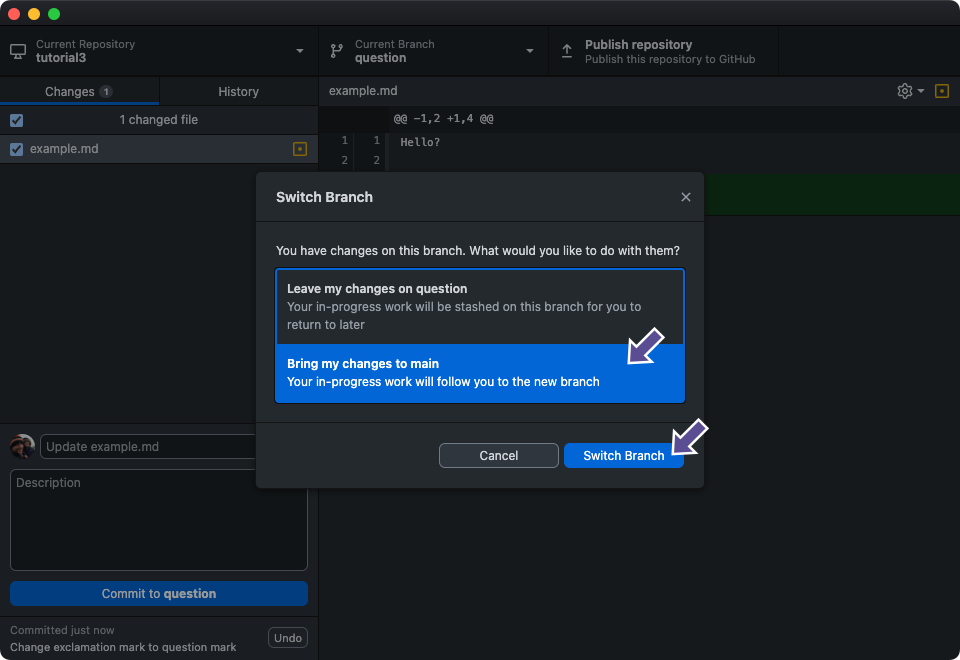
\includegraphics{images/image40.png}

And now if we look at the file, we'll see our stashed change has been
applied, but no question mark as this change still resides on the
\texttt{question} branch:

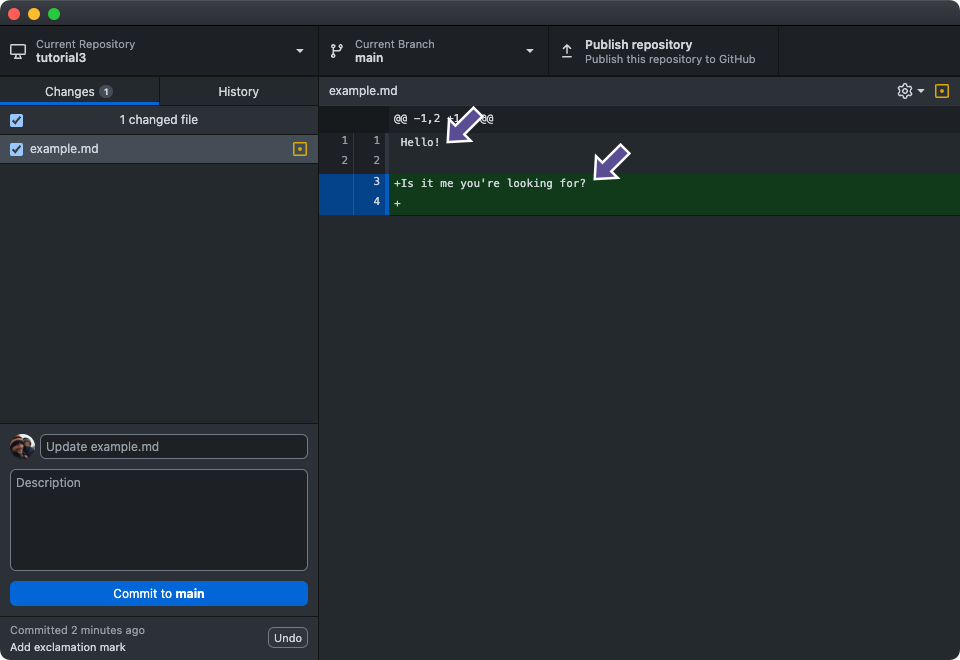
\includegraphics{images/image41.png}

Let's stage and commit our 2nd line:

\subsection{Command-line}

\begin{Shaded}
\begin{Highlighting}[]
\NormalTok{git add example.md}
\end{Highlighting}
\end{Shaded}

\begin{verbatim}
git commit -m "Add 2nd line"
[main 6859b82] Add 2nd line
1 file changed, 2 insertions(+)
\end{verbatim}

\subsection{GitHub Desktop}

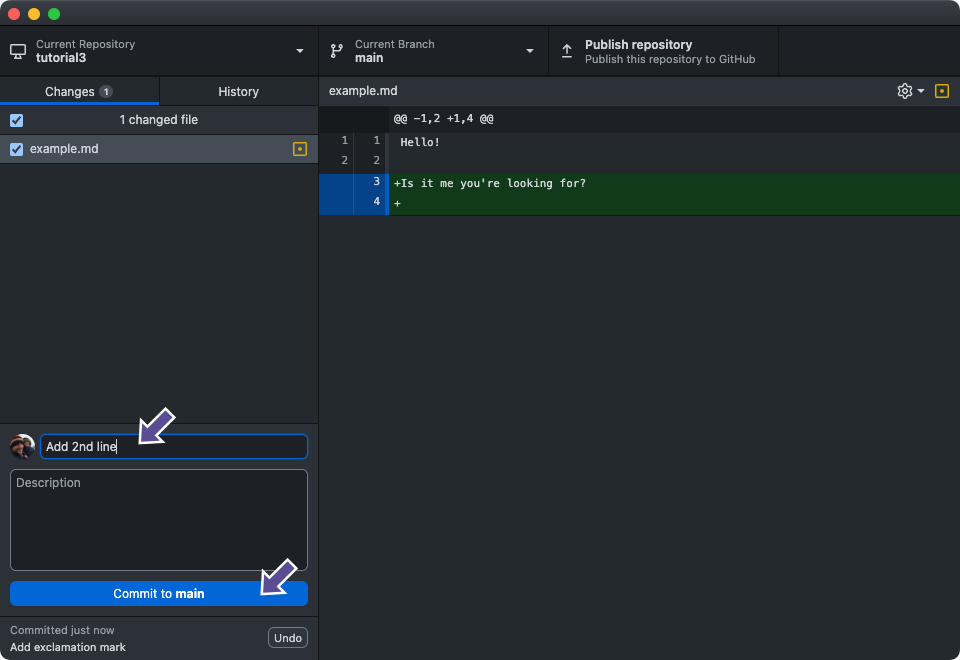
\includegraphics{images/image42.png}

Let's merge in the question mark.

\subsection{Command-line}

\begin{Shaded}
\begin{Highlighting}[]
\NormalTok{git merge question}
\end{Highlighting}
\end{Shaded}

\begin{verbatim}

Auto-merging example.md

Merge made by the 'ort' strategy.

example.md | 2 +-

1 file changed, 1 insertion(+), 1 deletion(-)
\end{verbatim}

\subsection{GitHub Desktop}

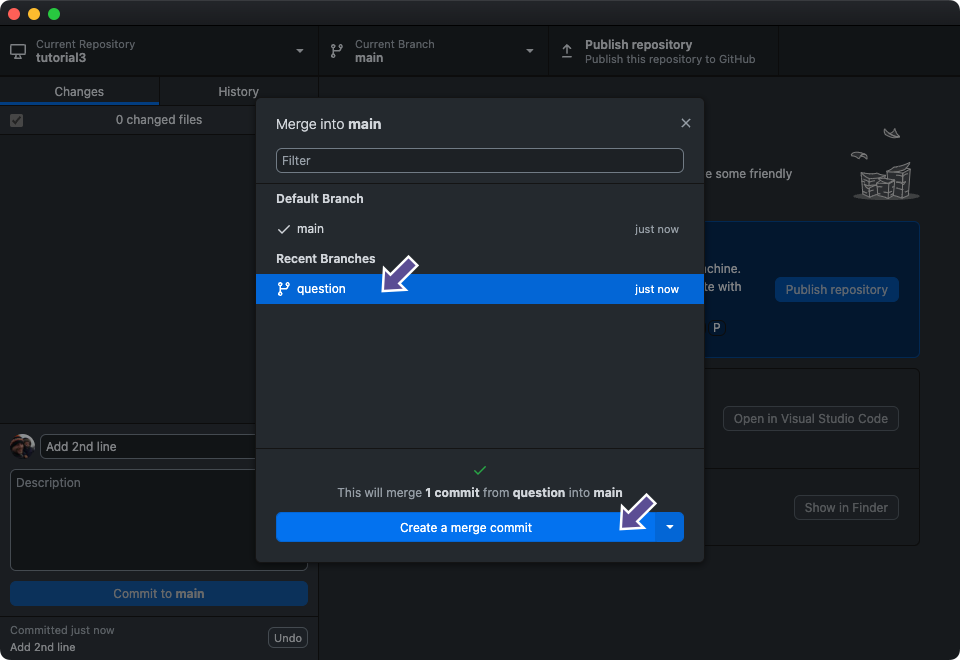
\includegraphics{images/image44.png}

Let's check the file:

\subsection{Command-line}

\begin{Shaded}
\begin{Highlighting}[]
\NormalTok{cat example.md}
\end{Highlighting}
\end{Shaded}

\begin{verbatim}

Hello?

Is it me you're looking for?
\end{verbatim}

\subsection{GitHub Desktop}

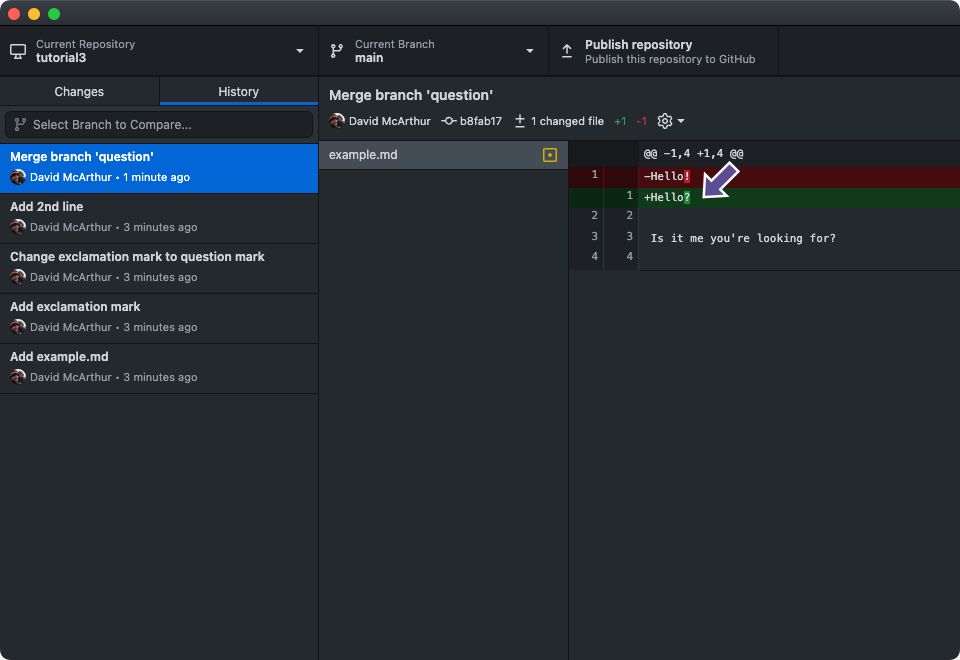
\includegraphics{images/image45.png}

\subsection{Merge conflicts}\label{merge-conflicts}

In the examples above we have introduced create a branch, making some
changes and then integrating this back into main. However, what happens
if you make a change to a line in a file on one branch, then you (or
someone else) changes the same line of the same file on a different
branch, what should Git do when you want to merge? This is a so-called
\textbf{merge conflict}.

In this section, we're going to create a simple scenario where we will
run into \textbf{merge conflicts} and explore two different ways to
resolve them.

When using \texttt{merge} to combine two branches, Git will first find a
common ``base commit'' between the two branches, then compare the
changes since this commit and attempt to compile a change list known as
a ``merge commit''.

Git tries to automate this process as much as possible, but if it finds
two conflicting changes it won't try to guess which change should
overrule the other. This usually happens when the same line in a file
has been changed in both branches. In this case, while attempting to
compile the merge commit, Git will go into a ``merge conflict'' state,
which involves updating the conflicting files in the filesystem (or
``working tree'') with some special formatting to show you what it
cannot guess, and Git will not allow you to commit the merge until you
have manually decided what you want to happen.

Let's create a branch named \texttt{capitalise} and switch to it:

\subsection{Command-line}

\begin{Shaded}
\begin{Highlighting}[]
\NormalTok{git }\ControlFlowTok{switch} \SpecialCharTok{{-}}\NormalTok{c capitalise}
\end{Highlighting}
\end{Shaded}

\begin{verbatim}
Switched to a new branch 'capitalise'
\end{verbatim}

\subsection{GitHub Desktop}

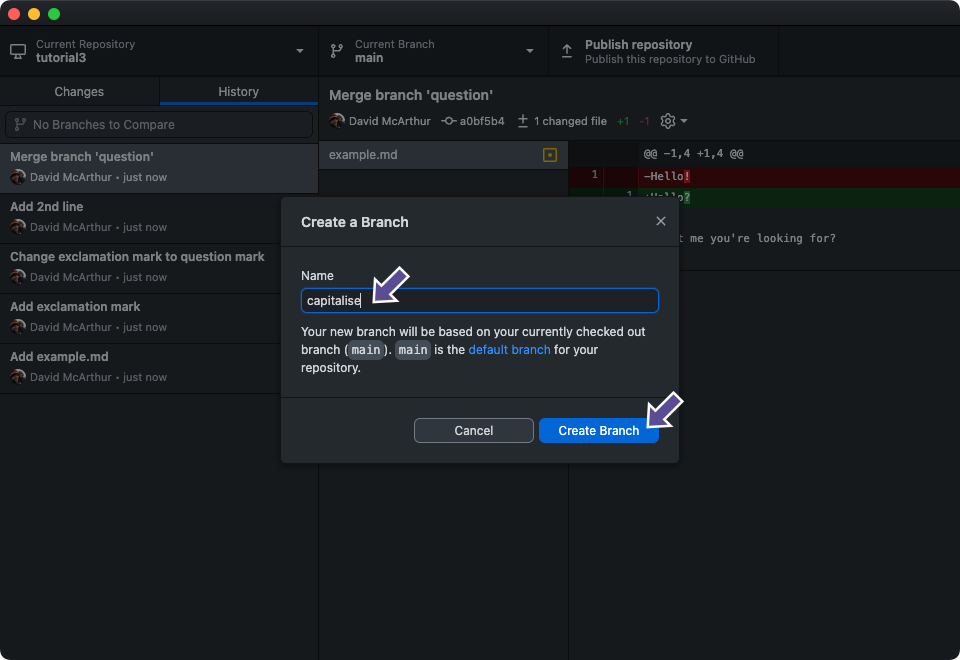
\includegraphics{images/image46_1.png}

Now we're going to make a different change to the file on the main
branch. This time change the contents to the following:

\begin{tcolorbox}[enhanced jigsaw, opacityback=0, colframe=quarto-callout-note-color-frame, toprule=.15mm, arc=.35mm, rightrule=.15mm, title=\textcolor{quarto-callout-note-color}{\faInfo}\hspace{0.5em}{example.md}, colbacktitle=quarto-callout-note-color!10!white, left=2mm, leftrule=.75mm, opacitybacktitle=0.6, toptitle=1mm, colback=white, bottomtitle=1mm, breakable, titlerule=0mm, bottomrule=.15mm, coltitle=black]

HELLO

\end{tcolorbox}

Then commit the change:

\subsection{Command-line}

\begin{Shaded}
\begin{Highlighting}[]
\NormalTok{git add example.md}
\NormalTok{git commit }\SpecialCharTok{{-}}\NormalTok{m }\StringTok{"Capitalise example.md"}
\end{Highlighting}
\end{Shaded}

\begin{verbatim}
[capitalise 3da9dfb] Capitalise example.md

1 file changed, 1 insertion(+), 3 deletions(-)
\end{verbatim}

\subsection{GitHub Desktop}

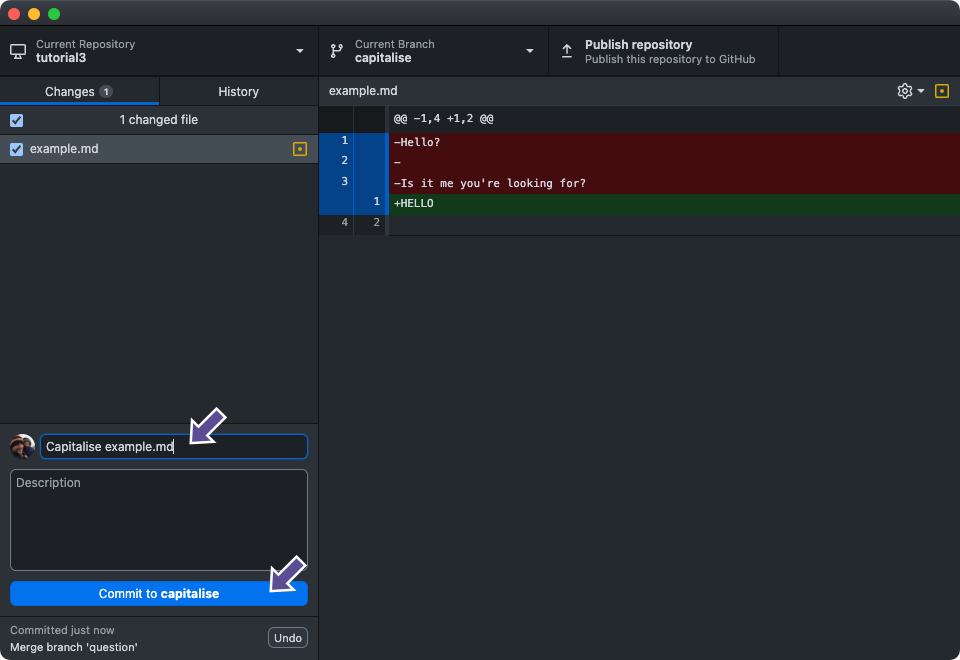
\includegraphics{images/image47.png}

Now switch back to the \texttt{main} branch:

\subsection{Command-line}

\begin{Shaded}
\begin{Highlighting}[]
\NormalTok{git }\ControlFlowTok{switch}\NormalTok{ main}
\end{Highlighting}
\end{Shaded}

\begin{verbatim}

Switched to branch 'main'
\end{verbatim}

\subsection{GitHub Desktop}

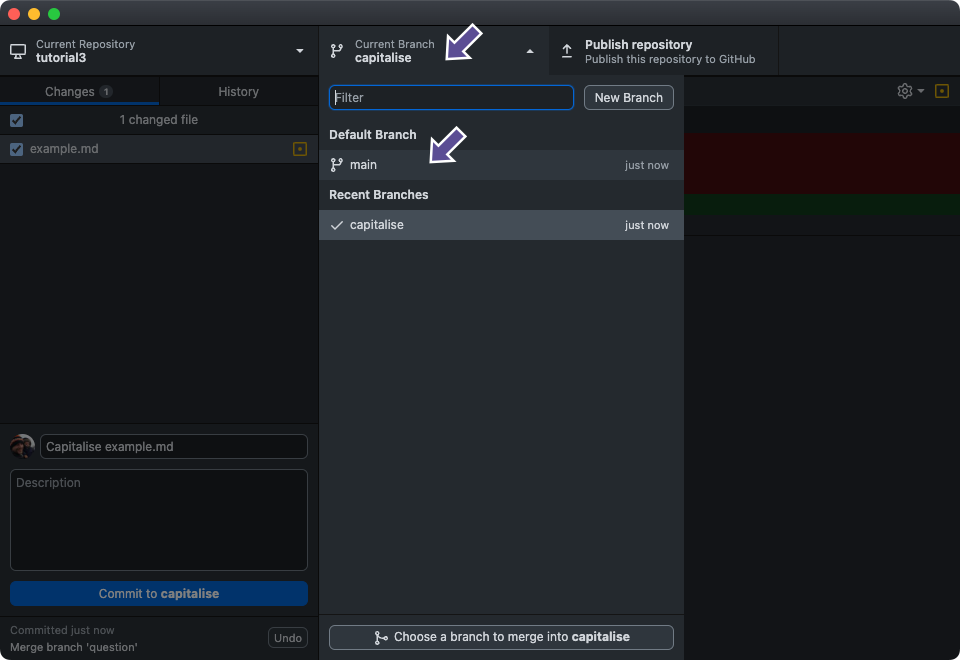
\includegraphics{images/image48.png}

The file should look like it did before the capitalisation, as that
change is isolated on the \texttt{capitalise} branch:

\subsection{Command-line}

\begin{Shaded}
\begin{Highlighting}[]
\NormalTok{cat example.md}
\end{Highlighting}
\end{Shaded}

\begin{verbatim}
Hello?

Is it me you're looking for?
\end{verbatim}

\subsection{GitHub Desktop}

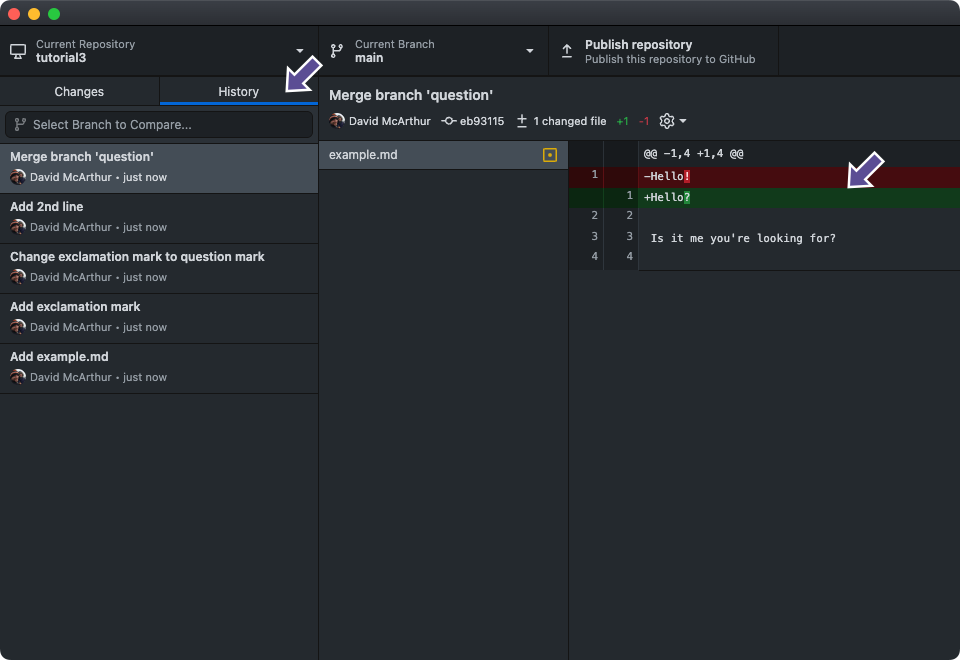
\includegraphics{images/image49.png}

Now we're going to make a different change to the file on the main
branch. This time change the contents to the following:

\begin{tcolorbox}[enhanced jigsaw, opacityback=0, colframe=quarto-callout-note-color-frame, toprule=.15mm, arc=.35mm, rightrule=.15mm, title=\textcolor{quarto-callout-note-color}{\faInfo}\hspace{0.5em}{example.md}, colbacktitle=quarto-callout-note-color!10!white, left=2mm, leftrule=.75mm, opacitybacktitle=0.6, toptitle=1mm, colback=white, bottomtitle=1mm, breakable, titlerule=0mm, bottomrule=.15mm, coltitle=black]

Hello.

\end{tcolorbox}

Stage and commit the change:

\subsection{Command-line}

\begin{Shaded}
\begin{Highlighting}[]
\NormalTok{git add example.md}
\NormalTok{git commit }\SpecialCharTok{{-}}\NormalTok{m }\StringTok{"Add full stop to end of the line in example.md"}
\end{Highlighting}
\end{Shaded}

\begin{verbatim}
[main 7888fef] Add full stop to end of the line in example.md

1 file changed, 1 insertion(+), 3 deletions(-)
\end{verbatim}

\subsection{GitHub Desktop}

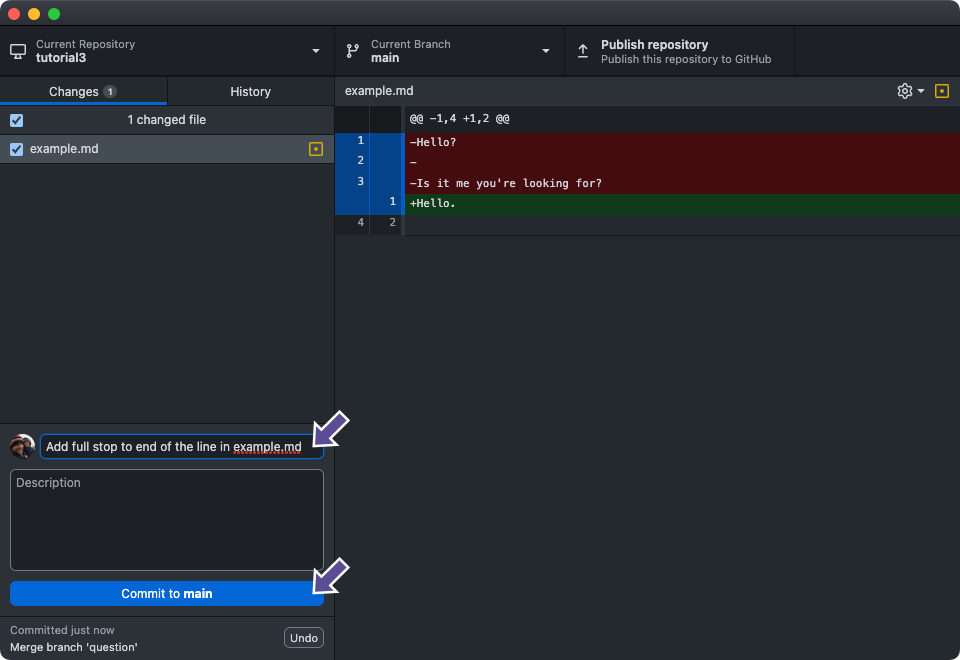
\includegraphics{images/image50.png}

Let's see what happens when we try to merge:

\subsection{Command-line}

\begin{Shaded}
\begin{Highlighting}[]
\NormalTok{git merge capitalise}
\end{Highlighting}
\end{Shaded}

\begin{verbatim}
Auto-merging example.md

CONFLICT (content): Merge conflict in example.md

Automatic merge failed; fix conflicts and then commit the result.
\end{verbatim}

\subsection{GitHub Desktop}

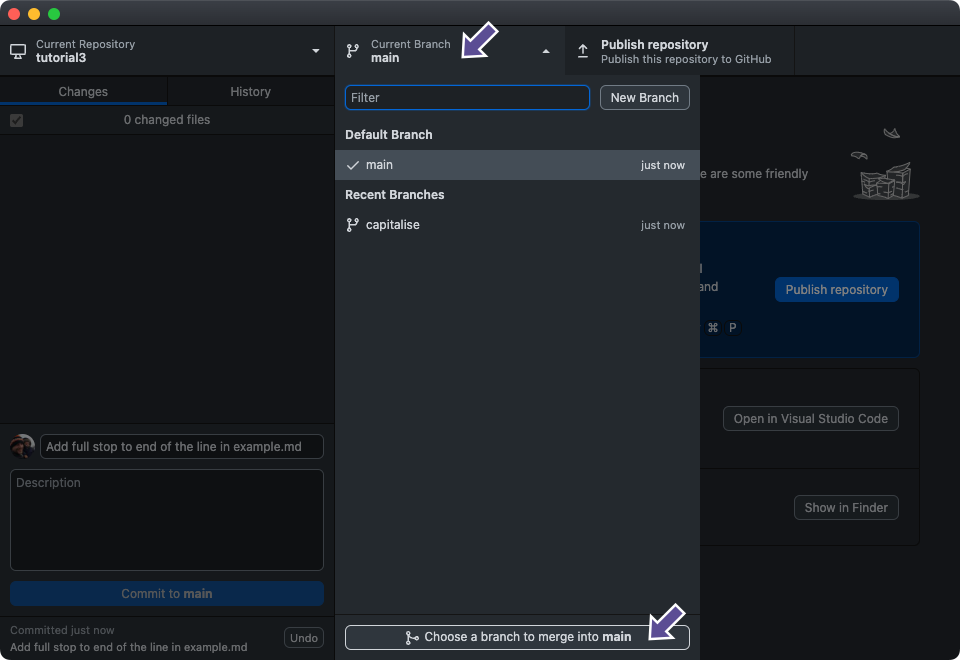
\includegraphics{images/image51.png}

Let's see what happens when we try to merge:

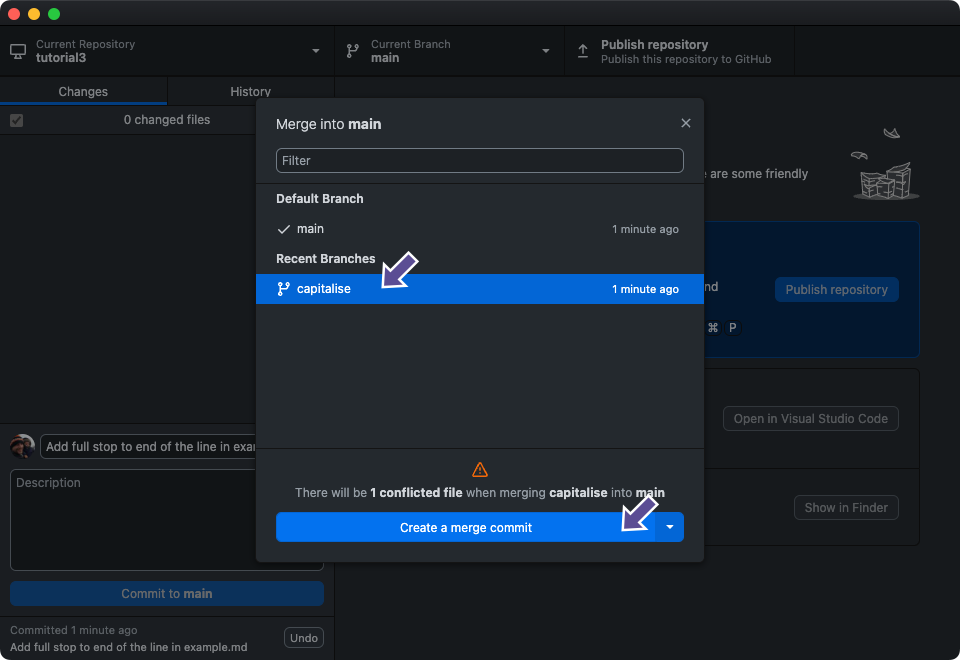
\includegraphics{images/image52.png}

Next, GitHub Desktop will tell you which files need attention, and
instruct you to open them in your preferred code editor.

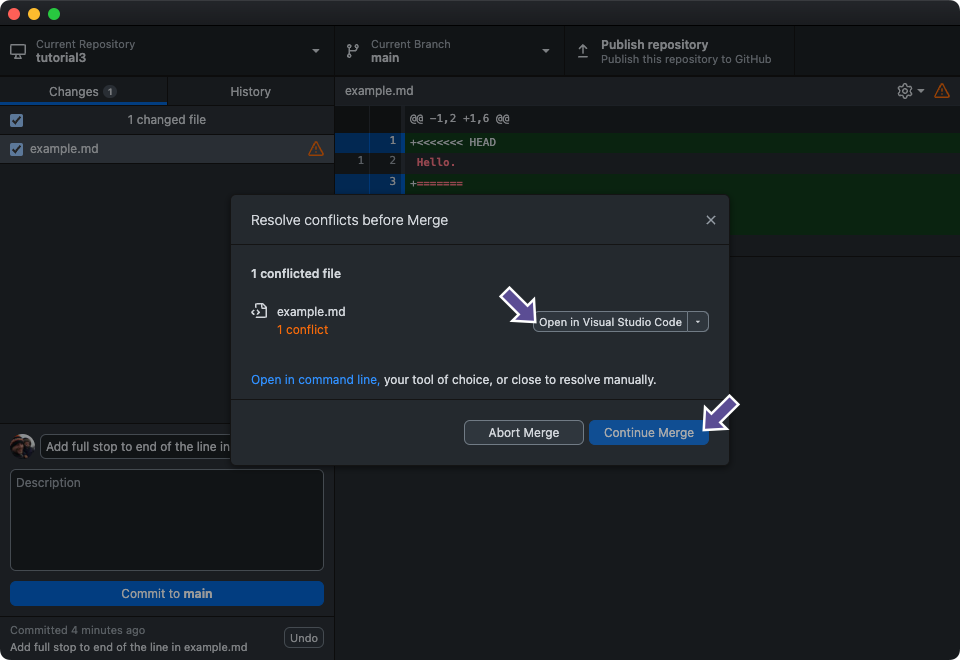
\includegraphics{images/image53.png}

The Continue Merge button is disabled, as we need to resolve the
conflicts in our files.

Let's open up \texttt{example.md} in our preferred editor and see what
is happening:

\begin{verbatim}

<<<<<<< HEAD

Hello.

=======

HELLO

>>>>>>> capitalise
\end{verbatim}

Git has modified our file to delineate a change that it cannot merge.
The line (or lines) between
\texttt{\textless{}\textless{}\textless{}\textless{}\textless{}\textless{}\textless{}}
and \texttt{======} here show what you already had (you can tell because
HEAD points to your current branch). The line (or lines) between
\texttt{=======} and
\texttt{\textgreater{}\textgreater{}\textgreater{}\textgreater{}\textgreater{}\textgreater{}\textgreater{}}
is what was introduced by the other commit, in this case from the
capitalise branch.

If this was a large file with multiple lines changed, Git will
automatically merge the parts that it can, and will highlight the parts
it can't like this, and we will have to go through each conflict and
manually resolve them.

Let's have a look at Git's status:

\subsection{Command-line}

\begin{Shaded}
\begin{Highlighting}[]
\NormalTok{git status }\SpecialCharTok{{-}}\NormalTok{v}
\end{Highlighting}
\end{Shaded}

\begin{verbatim}

On branch main

You have unmerged paths.

(fix conflicts and run "git commit")

(use "git merge --abort" to abort the merge)

Unmerged paths:

(use "git add <file>..." to mark resolution)

both modified:   example.md

* Unmerged path example.md

no changes added to commit (use "git add" and/or "git commit -a")
\end{verbatim}

\subsection{GitHub Desktop}

Note that GitHub Desktop displays the conflict icon besides each file
that needs attention:

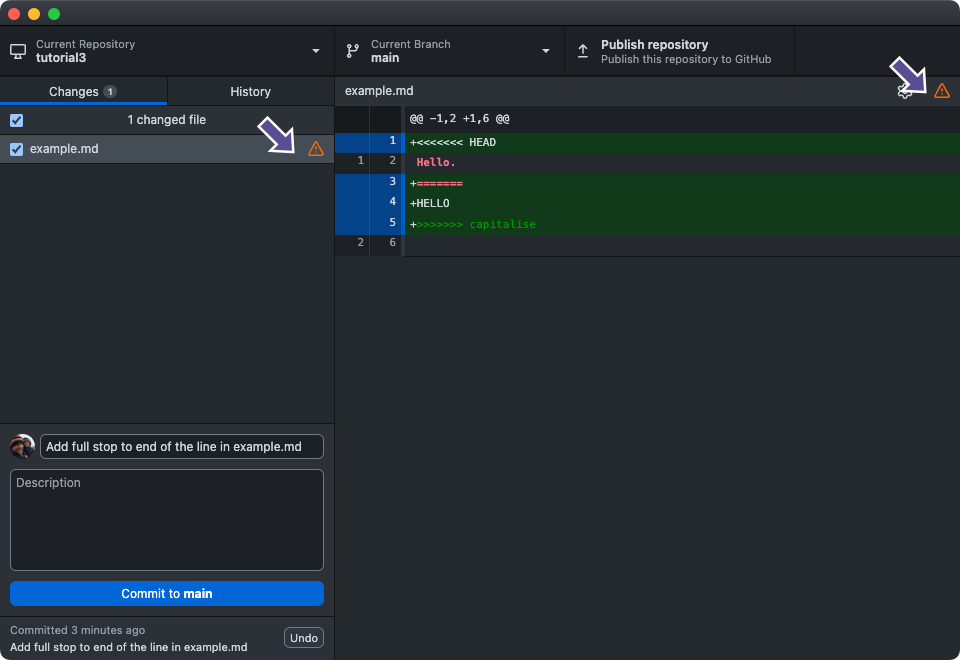
\includegraphics{images/image54.png}

Git's method for displaying merge conflicts by modifying the source
files makes it very straightforward for us to resolve, by just manually
editing the files as we want. However Git knows that there is now a
danger that you could commit this merge conflict syntax, and when
working with code, this will almost certainly cause a syntax error and
break your project. So Git tries to protect us against this by going
into a ``merge conflict'' state, where it wants you to either resolve or
abort this action before you do anything else.

Let's manually edit our file to what we want, like a mixture of both
changes:

\begin{tcolorbox}[enhanced jigsaw, opacityback=0, colframe=quarto-callout-note-color-frame, toprule=.15mm, arc=.35mm, rightrule=.15mm, title=\textcolor{quarto-callout-note-color}{\faInfo}\hspace{0.5em}{example.md}, colbacktitle=quarto-callout-note-color!10!white, left=2mm, leftrule=.75mm, opacitybacktitle=0.6, toptitle=1mm, colback=white, bottomtitle=1mm, breakable, titlerule=0mm, bottomrule=.15mm, coltitle=black]

HELLO.

\end{tcolorbox}

\subsection{Command-line}

Add the file to the stage to mark it as resolved:

\begin{Shaded}
\begin{Highlighting}[]
\NormalTok{git add example.md}
\end{Highlighting}
\end{Shaded}

We can see Git is no longer in a merge conflict state:

\begin{Shaded}
\begin{Highlighting}[]
\NormalTok{git status }\SpecialCharTok{{-}}\NormalTok{v}
\end{Highlighting}
\end{Shaded}

\begin{verbatim}

On branch main

All conflicts fixed but you are still merging.

(use "git commit" to conclude merge)

Changes to be committed:

modified:   example.md

diff --git a/example.md b/example.md

index 8b94e8e..c886167 100644

--- a/example.md

+++ b/example.md

@@ -1,2 +1,2 @@

-Hello.

+HELLO.
\end{verbatim}

\subsection{GitHub Desktop}

Once the special
\texttt{\textless{}\textless{}\textless{}\textless{}\textless{}\textless{}\textless{}},
\texttt{======} and
\texttt{\textgreater{}\textgreater{}\textgreater{}\textgreater{}\textgreater{}\textgreater{}\textgreater{}}
syntax is removed from our files, GitHub Desktop detects that our merge
conflict has been resolved and allows us to `Continue Merge':

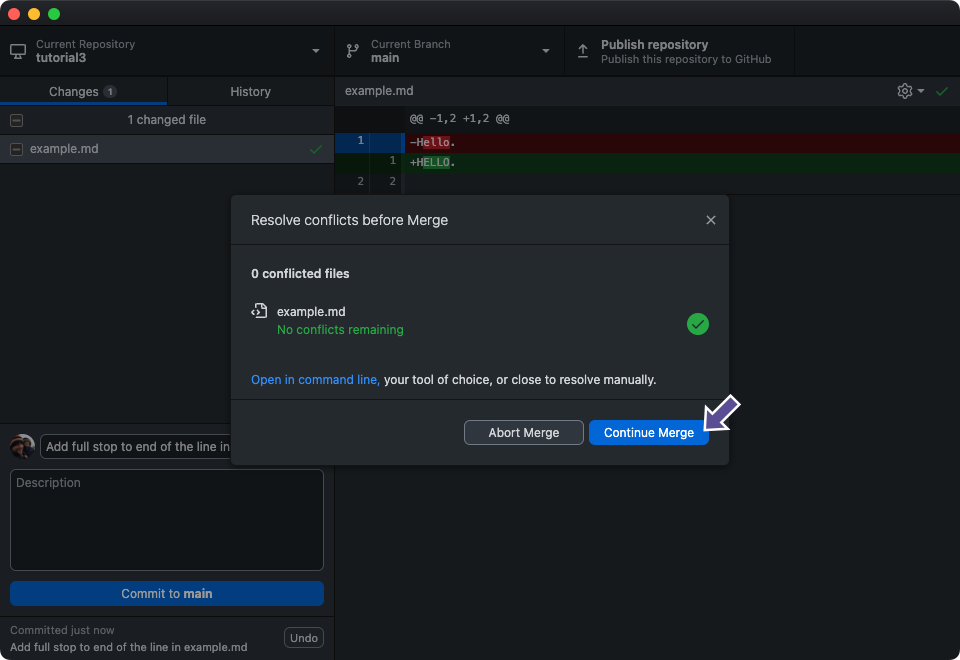
\includegraphics{images/image55.png}

And we can conclude the merge.

\subsection{Command-line}

I use the \texttt{-\/-no-edit} flag to tell Git to use the default
message for a merge commit:

\begin{Shaded}
\begin{Highlighting}[]
\NormalTok{git commit }\SpecialCharTok{{-}{-}}\NormalTok{no}\SpecialCharTok{{-}}\NormalTok{edit}
\end{Highlighting}
\end{Shaded}

\begin{verbatim}

[main fe2d762] Merge branch 'capitalise'
\end{verbatim}

\subsection{GitHub Desktop}

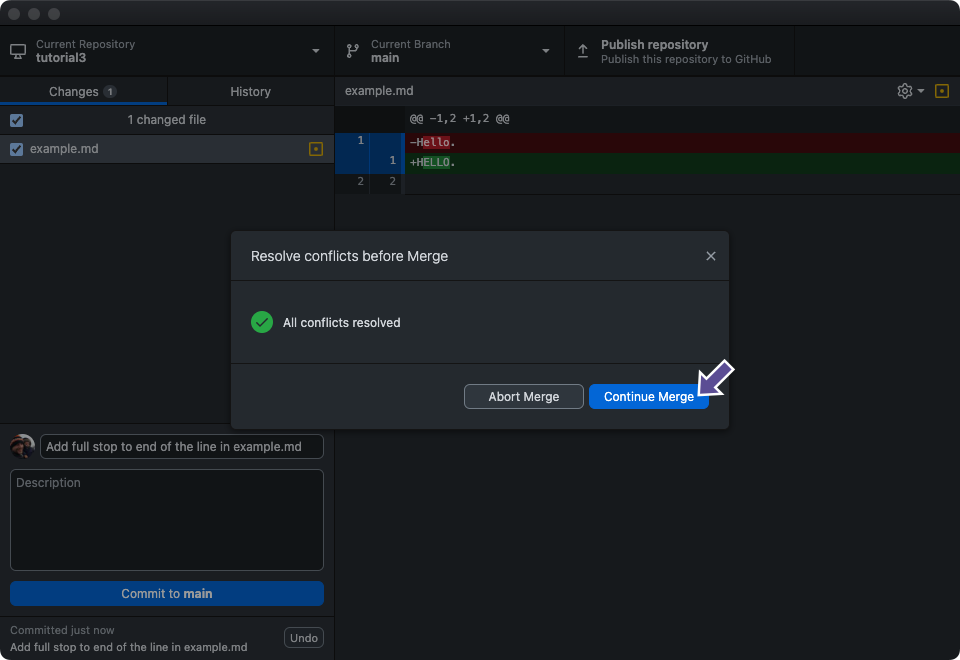
\includegraphics{images/image56.png}

We have integrated our branch into the \texttt{main} branch and we can
safely delete our short-lived branch \texttt{capitalise}:

\subsection{Command-line}

\begin{Shaded}
\begin{Highlighting}[]
\NormalTok{git branch }\SpecialCharTok{{-}{-}}\NormalTok{delete capitalise}
\end{Highlighting}
\end{Shaded}

\begin{verbatim}
Deleted branch capitalise (was 3da9dfb).
\end{verbatim}

\subsection{GitHub Desktop}

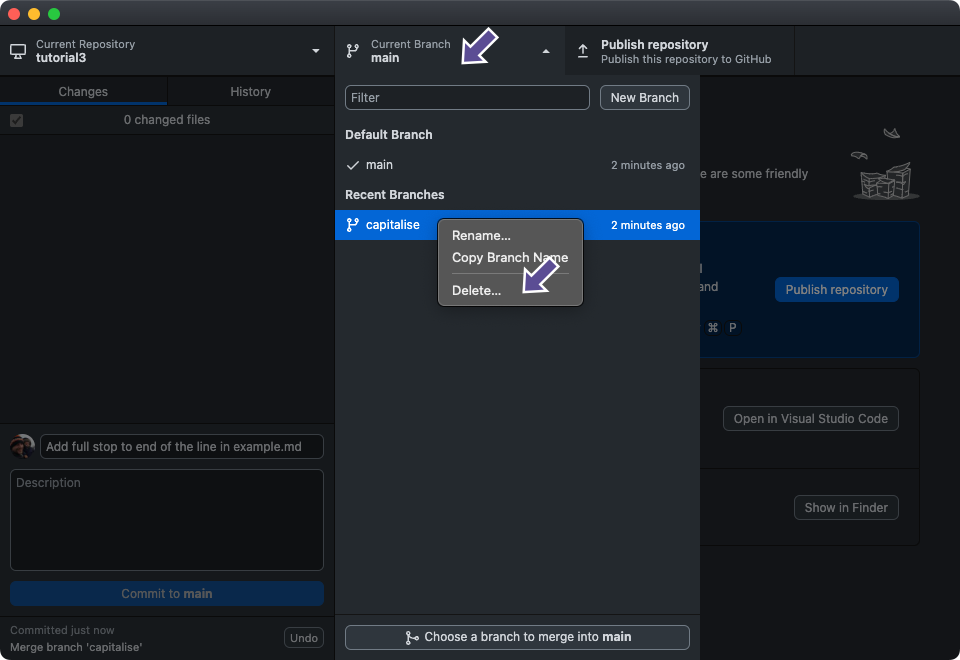
\includegraphics{images/image57.png}

\section{Code Review: A better approach to resolving merge
conflicts}\label{code-review-a-better-approach-to-resolving-merge-conflicts}

Although Git allows us to resolve a merge conflict as above, this is not
considered the ``best practice'' way to achieve this result. We ended up
with something different from both our branch contents and the main
branch contents all in one merge conflict resolution, with no
opportunity for oversight by someone else working on the project-
i.e.~we managed to skip the Code Review (aka. Pull Request) stage.

A Pull Request on GitHub should be thought of as a preparation and
checking stage for a Git \texttt{merge} (or \texttt{rebase}) operation.
GitHub needs a `base' branch to `merge into', usually \texttt{main}, and
a `compare' branch to `merge from'. If Git has indicated that a merge
will result in a merge conflict, for the base branch as above, GitHub
will not easily let you perform the merge process until this is fixed.
So let's see how this could have been done differently.

Let's create a new branch called \texttt{goodbye}:

\subsection{Command-line}

\begin{Shaded}
\begin{Highlighting}[]
\NormalTok{git }\ControlFlowTok{switch} \SpecialCharTok{{-}}\NormalTok{c goodbye}
\end{Highlighting}
\end{Shaded}

\begin{verbatim}
Switched to a new branch 'goodbye'
\end{verbatim}

\subsection{GitHub Desktop}

From the main menu select Branch \textgreater{} New Branch and name the
branch `goodbye': 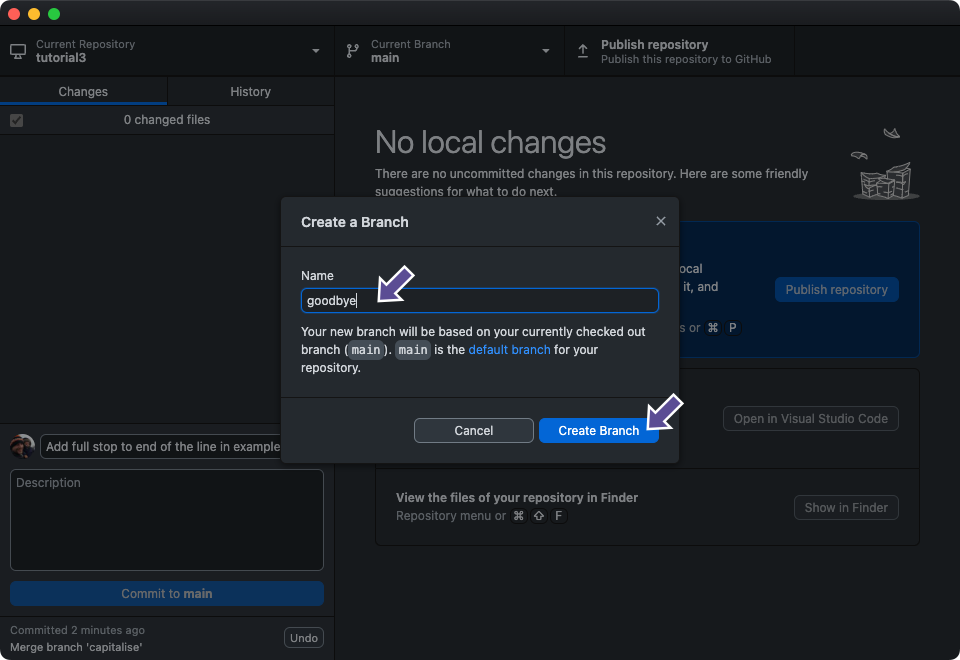
\includegraphics{images/image58.png}

Let's update the file like so:

\begin{tcolorbox}[enhanced jigsaw, opacityback=0, colframe=quarto-callout-note-color-frame, toprule=.15mm, arc=.35mm, rightrule=.15mm, title=\textcolor{quarto-callout-note-color}{\faInfo}\hspace{0.5em}{example.md}, colbacktitle=quarto-callout-note-color!10!white, left=2mm, leftrule=.75mm, opacitybacktitle=0.6, toptitle=1mm, colback=white, bottomtitle=1mm, breakable, titlerule=0mm, bottomrule=.15mm, coltitle=black]

GOODBYE

\end{tcolorbox}

And commit the change:

\subsection{Command-line}

\begin{Shaded}
\begin{Highlighting}[]
\NormalTok{git add example.md}
\NormalTok{git commit }\SpecialCharTok{{-}}\NormalTok{m }\StringTok{"Change hello to goodbye in example.md"}
\end{Highlighting}
\end{Shaded}

\begin{verbatim}
[goodbye 753e225] Change hello to goodbye in example.md
1 file changed, 1 insertion(+), 1 deletion(-)
\end{verbatim}

\subsection{GitHub Desktop}

From the main menu select Branch \textgreater{} New Branch and name the
branch `goodbye': 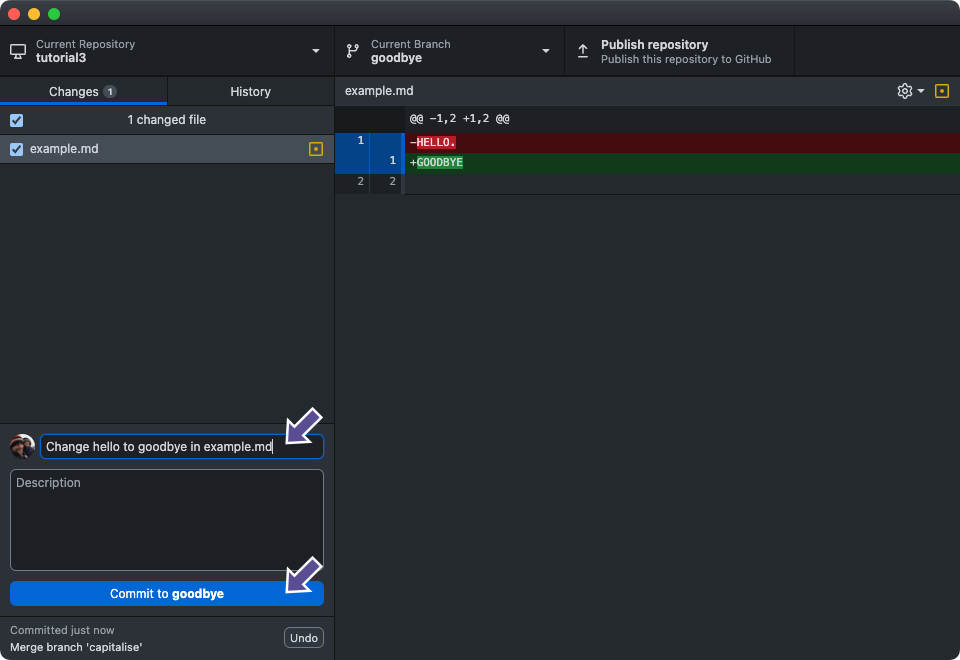
\includegraphics{images/image59.png}

Switch back to the main branch:

\subsection{Command-line}

\begin{Shaded}
\begin{Highlighting}[]
\NormalTok{git }\ControlFlowTok{switch}\NormalTok{ main}
\end{Highlighting}
\end{Shaded}

\begin{verbatim}
Switched to branch 'main'
\end{verbatim}

\subsection{GitHub Desktop}

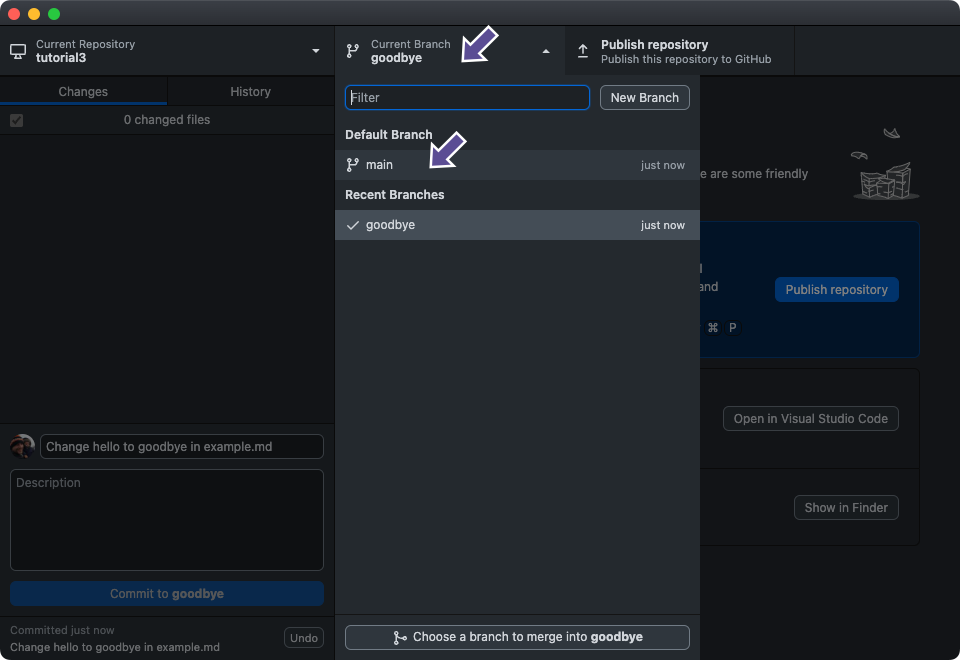
\includegraphics{images/image60.png}

Make a change to the file on the main branch:

\begin{tcolorbox}[enhanced jigsaw, opacityback=0, colframe=quarto-callout-note-color-frame, toprule=.15mm, arc=.35mm, rightrule=.15mm, title=\textcolor{quarto-callout-note-color}{\faInfo}\hspace{0.5em}{example.md}, colbacktitle=quarto-callout-note-color!10!white, left=2mm, leftrule=.75mm, opacitybacktitle=0.6, toptitle=1mm, colback=white, bottomtitle=1mm, breakable, titlerule=0mm, bottomrule=.15mm, coltitle=black]

HELLO

\end{tcolorbox}

And commit.

\subsection{Command-line}

\begin{Shaded}
\begin{Highlighting}[]
\NormalTok{git commit }\SpecialCharTok{{-}}\NormalTok{m }\StringTok{"Remove full stop in example.md"}
\end{Highlighting}
\end{Shaded}

\begin{verbatim}
[main 27c4cc0] Remove full stop in example.md
1 file changed, 1 insertion(+), 1 deletion(-)
\end{verbatim}

\subsection{GitHub Desktop}

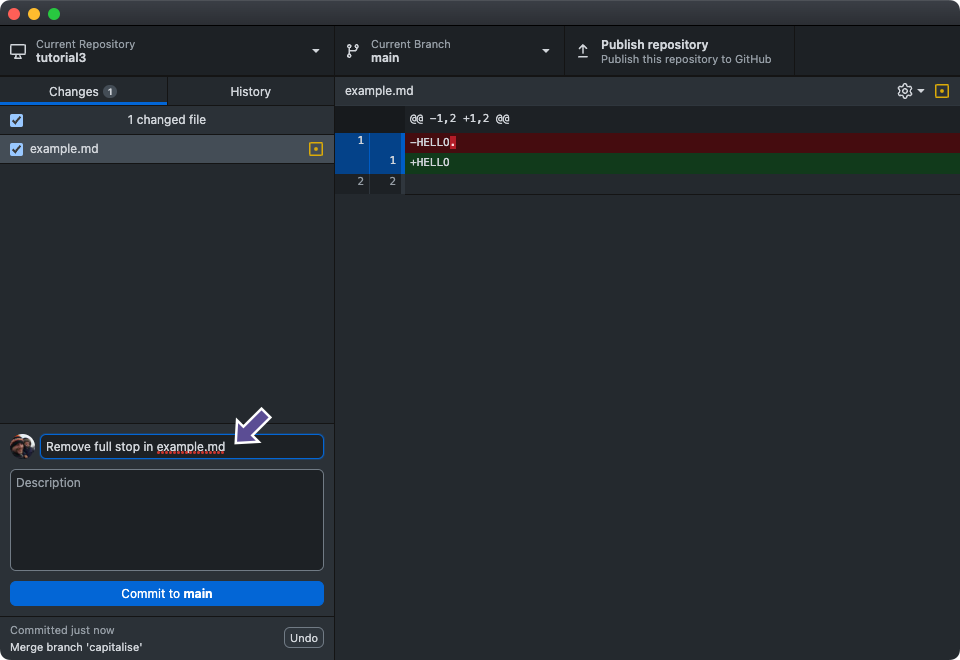
\includegraphics{images/image61.png}

Then try to merge:

\subsection{Command-line}

\begin{Shaded}
\begin{Highlighting}[]
\NormalTok{git merge goodbye}
\end{Highlighting}
\end{Shaded}

\begin{verbatim}
Auto-merging example.md
CONFLICT (content): Merge conflict in example.md
Automatic merge failed; fix conflicts and then commit the result.
\end{verbatim}

\subsection{GitHub Desktop}

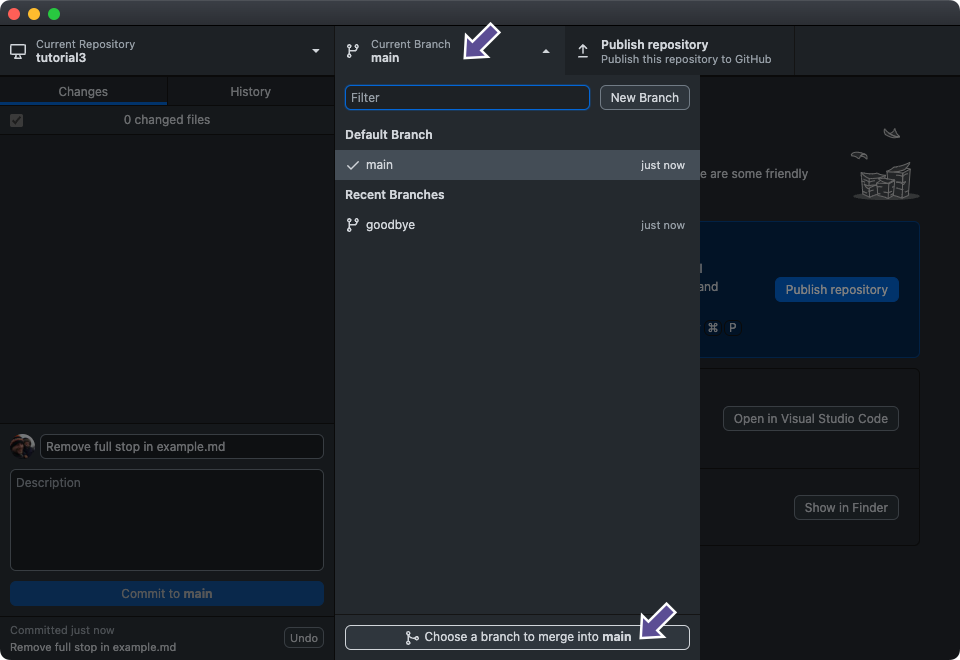
\includegraphics{images/image62.png}
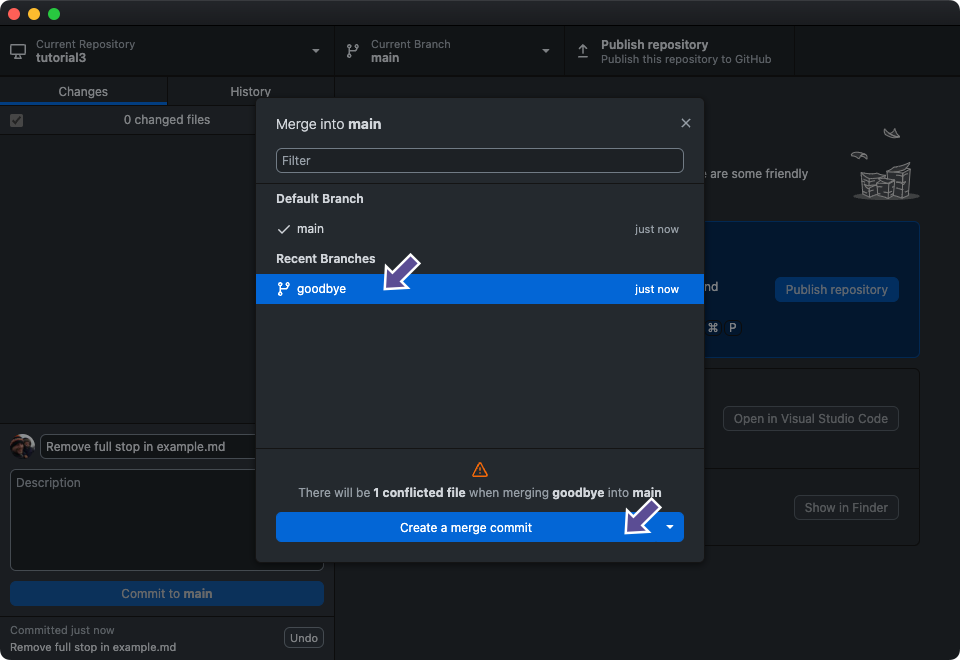
\includegraphics{images/image63.png}

And again we have a merge conflict. This time, let's abort the merge:

\subsection{Command-line}

\begin{Shaded}
\begin{Highlighting}[]
\NormalTok{git merge }\SpecialCharTok{{-}{-}}\NormalTok{abort}
\end{Highlighting}
\end{Shaded}

\subsection{GitHub Desktop}

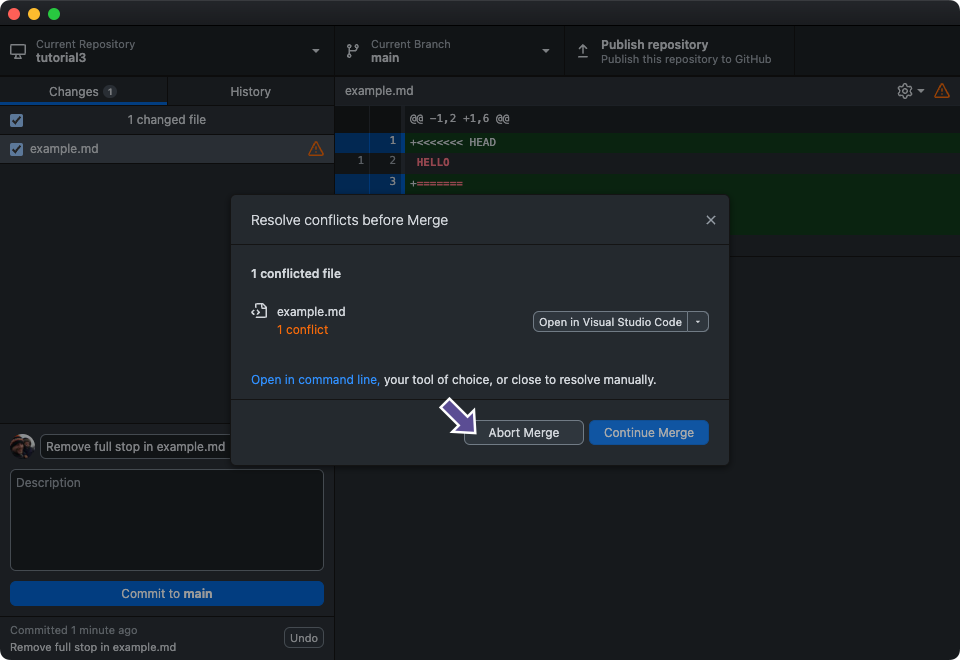
\includegraphics{images/image64.png}

Now switch back to the \texttt{goodbye} branch:

\subsection{Command-line}

\begin{Shaded}
\begin{Highlighting}[]
\NormalTok{git }\ControlFlowTok{switch}\NormalTok{ goodbye}
\end{Highlighting}
\end{Shaded}

\begin{verbatim}
Switched to branch 'goodbye'
\end{verbatim}

\subsection{GitHub Desktop}

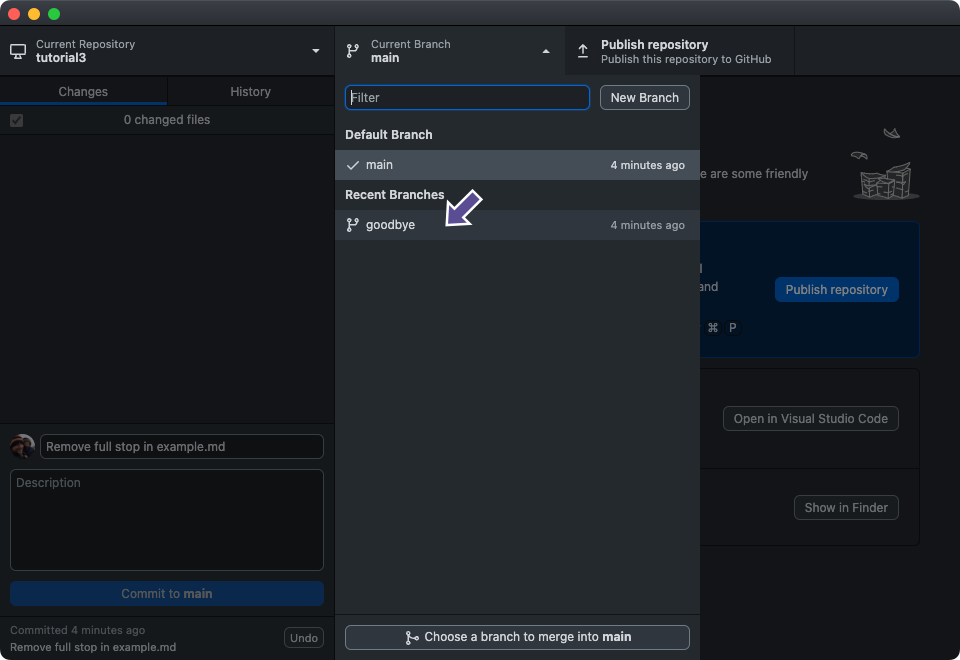
\includegraphics{images/image65.png}

And \textbf{merge \texttt{main} into our short-lived \texttt{goodbye}
branch}:

\subsection{Command-line}

\begin{Shaded}
\begin{Highlighting}[]
\NormalTok{git merge main}
\end{Highlighting}
\end{Shaded}

\begin{verbatim}
Auto-merging example.md
CONFLICT (content): Merge conflict in example.md
Automatic merge failed; fix conflicts and then commit the result.
\end{verbatim}

\subsection{GitHub Desktop}

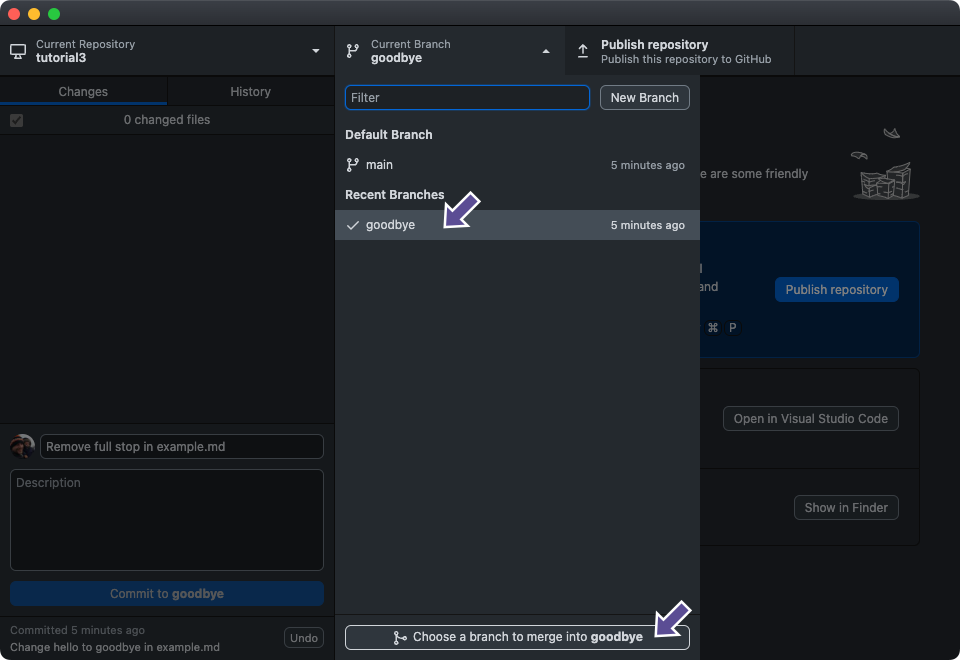
\includegraphics{images/image66.png}
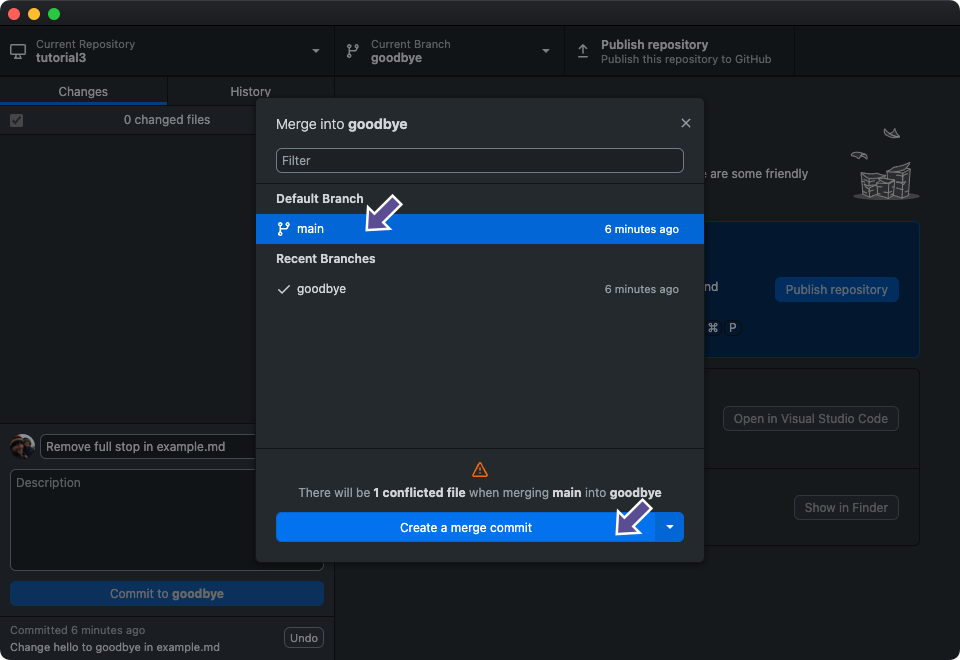
\includegraphics{images/image67.png}

Now if we head to our preferred code editor, we have almost the same
merge conflict to resolve (except \texttt{HEAD} is now our
\texttt{goodbye} branch):

\begin{verbatim}
<<<<<<< HEAD
GOODBYE
=======
HELLO
>>>>>>> main
\end{verbatim}

And we can manually resolve it as before, this time with some Beatles
lyrics:

\begin{tcolorbox}[enhanced jigsaw, opacityback=0, colframe=quarto-callout-note-color-frame, toprule=.15mm, arc=.35mm, rightrule=.15mm, title=\textcolor{quarto-callout-note-color}{\faInfo}\hspace{0.5em}{example.md}, colbacktitle=quarto-callout-note-color!10!white, left=2mm, leftrule=.75mm, opacitybacktitle=0.6, toptitle=1mm, colback=white, bottomtitle=1mm, breakable, titlerule=0mm, bottomrule=.15mm, coltitle=black]

You say GOODBYE and I say HELLO

\end{tcolorbox}

\subsection{Command-line}

And \texttt{add} to mark the conflict resolved:

\begin{Shaded}
\begin{Highlighting}[]
\NormalTok{git add example.md}
\end{Highlighting}
\end{Shaded}

And commit the change.

\begin{Shaded}
\begin{Highlighting}[]
\NormalTok{git commit }\SpecialCharTok{{-}{-}}\NormalTok{no}\SpecialCharTok{{-}}\NormalTok{edit}
\end{Highlighting}
\end{Shaded}

\begin{verbatim}
[goodbye 34ca84f] Merge branch 'main' into goodbye
\end{verbatim}

\subsection{GitHub Desktop}

GitHub Desktop has automatically detected that our merge conflict has
been resolved: 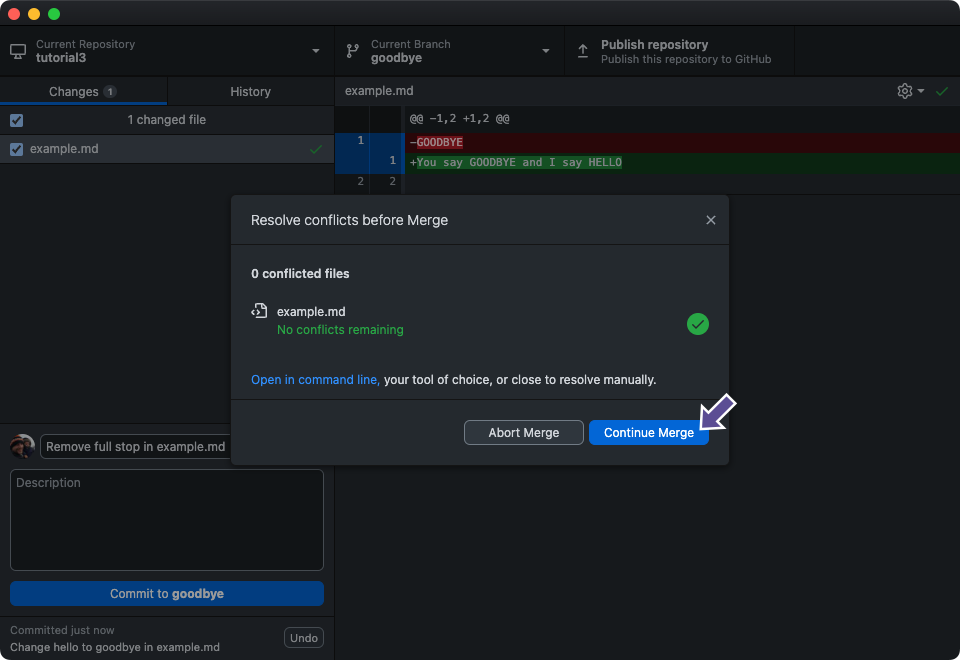
\includegraphics{images/image68.png}

\begin{tcolorbox}[enhanced jigsaw, opacityback=0, colframe=quarto-callout-note-color-frame, toprule=.15mm, arc=.35mm, rightrule=.15mm, title=\textcolor{quarto-callout-note-color}{\faInfo}\hspace{0.5em}{Note}, colbacktitle=quarto-callout-note-color!10!white, left=2mm, leftrule=.75mm, opacitybacktitle=0.6, toptitle=1mm, colback=white, bottomtitle=1mm, breakable, titlerule=0mm, bottomrule=.15mm, coltitle=black]

And now our branch could be ready for Code Review on GitHub via a Pull
Request (see Supplement). This makes sense when you are contributing to
someone else's project.

\end{tcolorbox}

When we switch back to the \texttt{main} branch:

\subsection{Command-line}

\begin{Shaded}
\begin{Highlighting}[]
\NormalTok{git }\ControlFlowTok{switch}\NormalTok{ main}
\end{Highlighting}
\end{Shaded}

\begin{verbatim}
Switched to branch 'main'
\end{verbatim}

\subsection{GitHub Desktop}

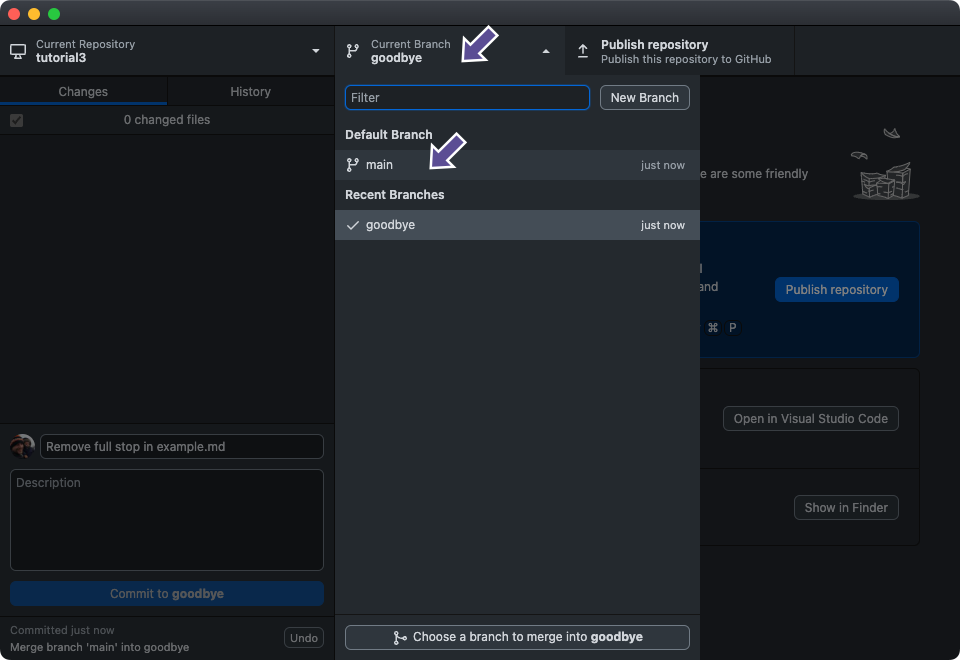
\includegraphics{images/image69.png}

Our change can be merged without a conflict. We will use
\texttt{git\ squash} in the next steps. Squashing allows you to combine
multiple commits in your branch's history into a single commit. This can
help keep your repository's history more readable and understandable.

\subsection{Command-line}

``Fast-forward'' in Git terms means an automatic merge, or in other
words, our merge will not result in a conflict.

The \texttt{goodbye} branch has 2 commits, which we can see by asking
\texttt{git\ log} to compare it to the \texttt{main} branch:

\begin{Shaded}
\begin{Highlighting}[]
\NormalTok{git log }\SpecialCharTok{{-}{-}}\NormalTok{oneline main..goodbye}
\end{Highlighting}
\end{Shaded}

\begin{verbatim}
34ca84f Merge branch 'main' into goodbye
753e225 Change hello to goodbye in example.md
\end{verbatim}

Since we resolved the merge conflict with Beatles lyrics when merging
the \texttt{main} branch into the \texttt{goodbye} branch, neither of
these commit messages does a good job describing what we are about to
integrate into \texttt{main}. So instead of transferring both commits to
the \texttt{main} `as is', let's `squash' them into one:

\begin{Shaded}
\begin{Highlighting}[]
\NormalTok{git merge }\SpecialCharTok{{-}{-}}\NormalTok{squash goodbye}
\end{Highlighting}
\end{Shaded}

\begin{verbatim}
Updating 27c4cc0..34ca84f
Fast-forward
Squash commit -- not updating HEAD
example.md | 2 +-
1 file changed, 1 insertion(+), 1 deletion(-)
\end{verbatim}

Then commit the squashed change with a more descriptive message:

\begin{Shaded}
\begin{Highlighting}[]
\NormalTok{git commit }\SpecialCharTok{{-}}\NormalTok{m }\StringTok{\textquotesingle{}Change to Beatles lyrics\textquotesingle{}}
\end{Highlighting}
\end{Shaded}

\begin{verbatim}
[main 08a1ff2] Change to Beatles lyrics
1 file changed, 1 insertion(+), 1 deletion(-)
\end{verbatim}

\subsection{GitHub Desktop}

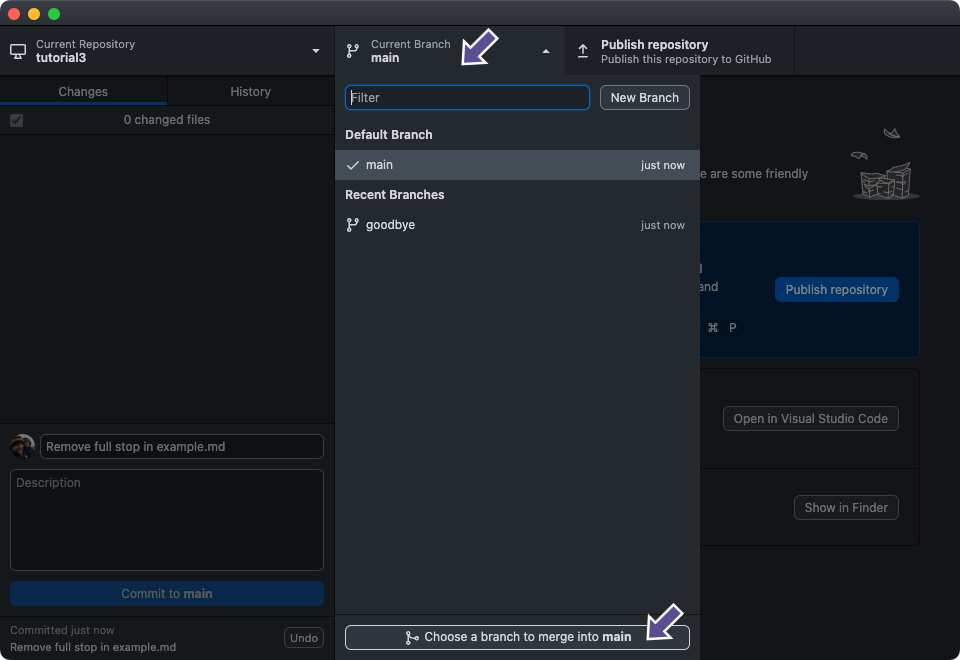
\includegraphics{images/image70.png}
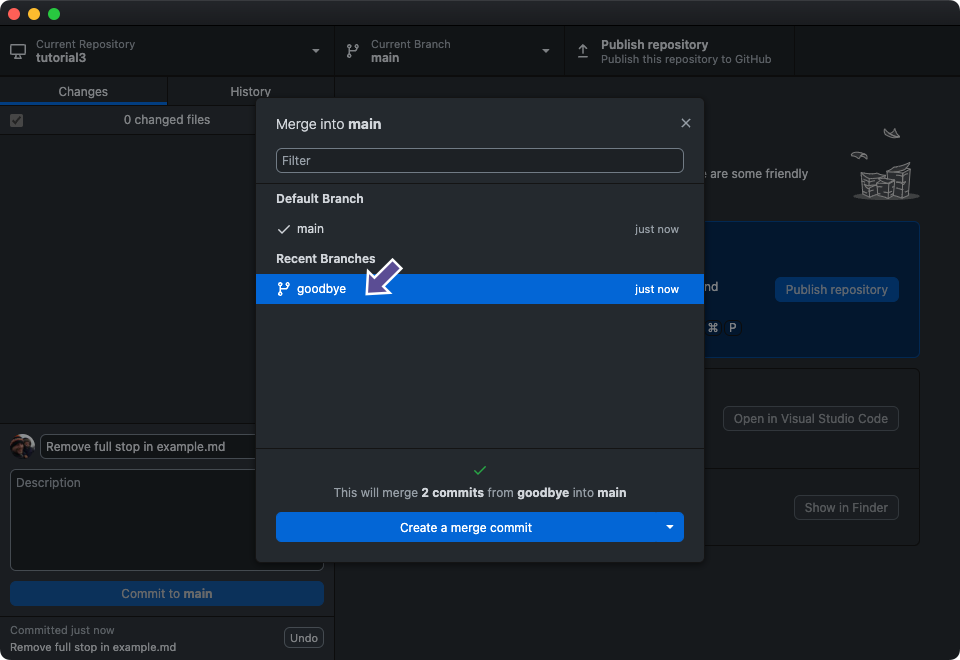
\includegraphics{images/image71.png}

This time instead of clicking `Create a merge commit', click the little
arrow on the right of the button and select `Squash and merge':

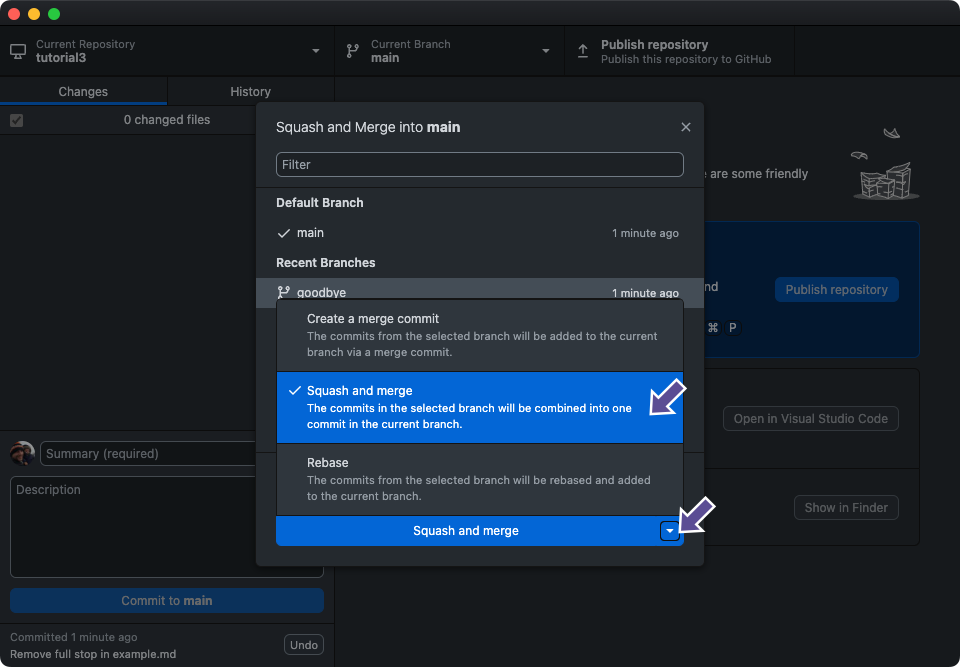
\includegraphics{images/image72.png}

Now if we look at the history tab we can see a commit with the message
`Squashed commit of the following:'. If you click on `Expand' on the
right, we can see the description of the commit has a log of the commits
that were squashed into this one:

\includegraphics{images/image73.png}

Let's change the title to something more descriptive by right-clicking
on the commit message and selecting `Amend commit\ldots{}':

\includegraphics{images/image74.png}

Then change the message to `Change to Beatles lyrics' and click `Amend
last commit':

\includegraphics{images/image75.png}

``Fast-forward'' in Git terms means an automatic merge, or in other
words, our merge will not result in a conflict.

Finally, you can safely delete the goodbye branch:

\subsection{Command-line}

\begin{Shaded}
\begin{Highlighting}[]
\NormalTok{git branch }\SpecialCharTok{{-}{-}}\NormalTok{delete goodbye}
\end{Highlighting}
\end{Shaded}

\begin{verbatim}
error: The branch 'goodbye' is not fully merged.
If you are sure you want to delete it, run 'git branch -D goodbye'.
\end{verbatim}

\subsection{GitHub Desktop}

\includegraphics{images/image76.png}

So to recap, we have prepared our branch for integration by first
combining any new changes from the \texttt{main} branch into our branch
and resolving the merge conflicts in isolation, creating a ``final
version'' of the change we want to make with our branch ready to be
checked, before attempting to integrate our branch back into the
\texttt{main} branch.

If you need to keep your short-lived branch open for some reason, it's
advised to merge any recent changes from \texttt{main} into your branch
often, to avoid painful merge conflicts later.

\section{Supplement: Create a Pull Request to an existing
project}\label{supplement-create-a-pull-request-to-an-existing-project}

This tutorial is about contributing to someone else's project. The
sample project that we are going to contribute to can be found here:

\url{https://github.com/UofGAnalyticsData/tutorial2}

We're simply going to add a line to the existing readme.md file, but you
may have found a bug, or thought of a new feature, in someone else's
project, and you've taken it upon yourself to contribute and submit it
to the project maintainer for approval.

In Git terms, what you need to do is:

\begin{enumerate}
\def\labelenumi{\arabic{enumi}.}
\tightlist
\item
  \textbf{Fork} the project on GitHub to your account
\item
  \textbf{Clone} it to your local machine
\item
  Make the change
\item
  \textbf{Stage}, \textbf{commit} and \textbf{push} the change to GitHub
\item
  Create a \textbf{Pull Request} on the original project which points to
  your forked repository
\item
  \textbf{Code review}: the project maintainer will review your change
  to decide if they want to integrate it, close it, or request
  modifications
\end{enumerate}

\begin{tcolorbox}[enhanced jigsaw, opacityback=0, colframe=quarto-callout-note-color-frame, toprule=.15mm, arc=.35mm, rightrule=.15mm, title=\textcolor{quarto-callout-note-color}{\faInfo}\hspace{0.5em}{Note}, colbacktitle=quarto-callout-note-color!10!white, left=2mm, leftrule=.75mm, opacitybacktitle=0.6, toptitle=1mm, colback=white, bottomtitle=1mm, breakable, titlerule=0mm, bottomrule=.15mm, coltitle=black]

What is the difference between Clone and Fork?

\textbf{Clone} is a Git feature that allows a user to make a copy of a
repository, including all the associated metadata on their computer so
they can work on it. This is an essential feature and makes sense for a
team of collaborators, with read-and-write privileges to the repository,
all working on a project together.

If you have read privileges but not write privileges to a repository,
like for example an open-source GitHub project where you're not a
project maintainer like the
\href{https://github.com/facebook/react}{React} repository we explored
above, it's easy to consume open-source projects but difficult to
contribute to them.

\textbf{Fork} is a GitHub feature aimed at making it easier to be part
of the open-source community. When you fork a repository, you make a
copy of a repository, including all the associated metadata, but
crucially, you become the owner of the new copied repository, and you
now have read and write privileges necessary to make changes.

If you would like to contribute your changes back to the original
repository, you can create a \textbf{Forked Pull Request} (see the next
section) which will notify the original project maintainers that you are
requesting to have your changes integrated with their project. Those
maintainers reserve the right to approve, reject, or request changes to
your Pull Request.

\end{tcolorbox}

\subsection{Fork}\label{fork}

To fork a GitHub repository, first, click the Fork button on the top
right:

\includegraphics{images/image77.png}

Then you have the opportunity to give the forked repository a different
name, description, and which branch to fork:
\includegraphics{images/image78.png}

And that's it! You have a copy of the project under your name on GitHub:

\subsection{Clone}\label{clone-1}

Next, we'll clone the project to our local machine:

\subsection{Command-line}

\includegraphics{images/image80_1.png}

\begin{enumerate}
\def\labelenumi{\arabic{enumi}.}
\tightlist
\item
  Click on the green button labelled ``Code''
\item
  Choose either HTTPS or SSH depending on your authentication setup and
  copy the URL Next, we can navigate to the folder we want and run the
  command:
\end{enumerate}

\begin{Shaded}
\begin{Highlighting}[]
\NormalTok{git clone git}\SpecialCharTok{@}\NormalTok{github.com}\SpecialCharTok{:}\NormalTok{daviestar}\SpecialCharTok{/}\NormalTok{tutorial2.git .}
\end{Highlighting}
\end{Shaded}

\begin{verbatim}
Cloning into '.'...
\end{verbatim}

\subsection{GitHub Desktop}

In GitHub Desktop, click on the `repository' tab in the top-left of the
window, then `Add', then `Clone repository\ldots{}':
\includegraphics{images/image80.png}

Choose the `URL' tab and enter \texttt{dmca-glasgow/tutorial2} into the
`Repository URL' input box, choose where you'd like to store the
repository on your computer, then finally click `Clone':
\includegraphics{images/image81.png}

\subsection{Make some changes}\label{make-some-changes}

Let's add a new line to the \texttt{readme.md} file, making sure to save
it:

\begin{tcolorbox}[enhanced jigsaw, opacityback=0, colframe=quarto-callout-note-color-frame, toprule=.15mm, arc=.35mm, rightrule=.15mm, title=\textcolor{quarto-callout-note-color}{\faInfo}\hspace{0.5em}{readme.md}, colbacktitle=quarto-callout-note-color!10!white, left=2mm, leftrule=.75mm, opacitybacktitle=0.6, toptitle=1mm, colback=white, bottomtitle=1mm, breakable, titlerule=0mm, bottomrule=.15mm, coltitle=black]

\#\# Follow along tutorial 2: Create a Pull Request to an existing
project

My updated text.

\end{tcolorbox}

\subsection{Stage, commit and push the change to our
repository}\label{stage-commit-and-push-the-change-to-our-repository}

\subsection{Command-line}

\begin{Shaded}
\begin{Highlighting}[]
\NormalTok{git add readme.md}
\NormalTok{git commit }\SpecialCharTok{{-}}\NormalTok{m }\StringTok{"added my updated text to readme"}
\NormalTok{git push}
\end{Highlighting}
\end{Shaded}

\begin{verbatim}
[main 7d73c6c] added my updated text to readme
1 file changed, 2 insertions(+)
To github.com:daviestar/tutorial2.git
c9dfc4a..7d73c6c  main -> main
\end{verbatim}

\subsection{GitHub Desktop}

In GitHub Desktop, add a descriptive message and click `Commit to main':
\includegraphics{images/image82.png}

\subsection{Create a Pull Request}\label{create-a-pull-request}

\includegraphics{images/image83.png}

\begin{enumerate}
\def\labelenumi{\arabic{enumi}.}
\tightlist
\item
  Navigate to the original project repository
\item
  Click on the Pull Requests tab
\item
  Click on the green button with the label ``New pull request''
\end{enumerate}

\includegraphics{images/image84.png}

\begin{enumerate}
\def\labelenumi{\arabic{enumi}.}
\tightlist
\item
  Click ``compare across forks''
\item
  Select your repository from the ``head'' dropdown menu
\item
  See your commit message!
\item
  See the contents of your commit! Now you can click the green button
  with the label ``Create pull request''.
\end{enumerate}

\includegraphics{images/image85.png}

Now you have the opportunity to rename your Pull Request and give it a
description. When you're ready, you can click the green button with the
label ``Create pull request''.

Note that you have the option to create a ``Draft Pull Request''. This
lets other users know that although you have opened a Pull Request, it's
not ready to review yet. This allows you the flexibility to set up the
Pull Request before finalising the change. For example, you may want to
make others aware that you are working on this particular change so they
don't start working on it too.

The ``Draft Pull Request'' feature is unfortunately only available on
public repositories and some enterprise accounts. If you were hoping to
use this workflow in a private repository, another convention is to put
``WIP'' (Work In Progress) at the top of your Pull Request description.

\includegraphics{images/image86.png}

Now we can see our Pull Request has been created. At this point, the
project maintainers will be notified. There's nothing else we can do
now, as we don't have permission to integrate this change ourselves, but
we will be notified if there is any activity on the Pull Request.

\subsection{Code review}\label{code-review}

The Pull Request page we have just created is where a project maintainer
will perform a code review. As an extreme example, the reviewer has a
duty to at least ensure someone isn't submitting a virus to their
project, so your code \emph{will} be read and reviewed.

For the reviewer, this is a whole topic (or even course) on its own as
Code Review can be such a powerful process. At its best, it can be an
opportunity to spread knowledge and build relationships in a team while
keeping the codebase standardised and robust. It's just simply a good
idea to have a 2nd set of eyes look over your code offering constructive
criticism.



\end{document}
